%%%%%%%%%%%%%%%%%%%%%%%%%%%%%%%%%%%%%%%%%%%%%%%%%%%%%%%%%%%%%%%%%%%%%%%%%%%%
%% Author template for Operations Reseacrh (opre) for articles with no e-companion (EC)
%% Mirko Janc, Ph.D., INFORMS, mirko.janc@informs.org
%% ver. 0.95, December 2010
%%%%%%%%%%%%%%%%%%%%%%%%%%%%%%%%%%%%%%%%%%%%%%%%%%%%%%%%%%%%%%%%%%%%%%%%%%%%
\documentclass[fleqn,mnsc,nonblindrev]{informs4}
%%\documentclass[opre,nonblindrev]{informs3_modified} % current default for manuscript submission

\usepackage{xr}
\makeatletter
\newcommand*{\addFileDependency}[1]{
\typeout{(#1)}
\@addtofilelist{#1}
\IfFileExists{#1}{}{\typeout{No file #1.}}
}\makeatother
\newcommand*{\myexternaldocument}[1]{%
\externaldocument{#1}%
\addFileDependency{#1.tex}%
\addFileDependency{#1.aux}%
}
\myexternaldocument{1Revisedmain}


\usepackage{fix-cm}
\usepackage{setspace}
\usepackage{booktabs}
\usepackage{pgfplots}
\usepgfplotslibrary{fillbetween}
\pgfplotsset{compat=1.18}
\usepackage{adjustbox}


% caption package

\makeatletter
\long\def\@makefigurecaption#1#2{\EGT\FigureCaptionFontStyle
\FigureNameFontStyle #1\ \ignorespaces #2\HD{0}{9}\endgraf}
\makeatother
\makeatletter
\long\def\@maketablecaption#1#2{\EGT\TableCaptionFontStyle
\noindent\textbf{#1} #2\par}
\makeatother

\usepackage{subcaption}
\captionsetup[sub]{font=small,labelfont={bf,sf}}

\usepackage[font=small, margin=1cm]{caption}

% Commands---------------------------------------

\newcommand{\ex}[1]{\mathbb{E}\left[#1\right]}
\newcommand{\Normal}{\operatorname{Normal}}
\newcommand{\CE}{\operatorname{CE}}
\newcommand{\EE}{\mathbb{E}}
\newcommand{\QQ}{\mathbb{Q}}
\newcommand{\PP}{\mathbb{P}}
\newcommand{\Var}{\operatorname{Var}}
\newcommand{\Cov}{\operatorname{Cov}}
\newcommand{\bs}{\bigskip}
\newcommand{\var}[2]{\mathrm{VaR}_{#1}(#2)}
\newcommand{\indi}[1]{\mathbb{I}_{\{#1\}}}
\newcommand{\prob}[1]{\mathbb{P}[#1]}
\newcommand{\ifn}[1]{\mathbbm{1}_{\{#1\}}}
\newcommand{\ig}[4]{\int_{#1}^{#2}\,#3\,\mathrm{d}{#4}}
\newcommand{\tvar}[2]{\mathrm{TVaR}_{#1}(#2)}
\newcommand{\com}[1]{{ \color{red} [#1] }}
\newcommand{\tb}[1]{\textbf{#1}}
\newcommand{\macom}[1]{{\color{purple}[#1]}}
\definecolor{darkpastelgreen}{rgb}{0.01, 0.75, 0.24}
\newcommand{\skcom}[1]{{\color{darkpastelgreen}[#1]}}
\newcommand{\ma}[1]{{\color{blue}#1}}
\newcommand{\blfootnote}[1]{
\begingroup
\renewcommand\thefootnote{}\footnote{#1}
\addtocounter{footnote}{-1}
\endgroup
}


\OneAndAHalfSpacedXI % current default line spacing
%\OneAndAHalfSpacedXII
%\DoubleSpacedXII
%%\DoubleSpacedXI

% If hyperref is used, dvi-to-ps driver of choice must be declared as
%   an additional option to the \documentclass. For example
%\documentclass[dvips,opre]{informs3}      % if dvips is used
%\documentclass[dvipsone,opre]{informs3}   % if dvipsone is used, etc.

%%% OPRE uses endnotes. If you do not use them, put a percent sign before
%%% the \theendnotes command. This template does show how to use them.
\usepackage{endnotes}
\let\footnote=\endnote
\let\enotesize=\normalsize
\def\notesname{Endnotes}%
\def\makeenmark{$^{\theenmark}$}
\def\enoteformat{\rightskip0pt\leftskip0pt\parindent=1.75em
\leavevmode\llap{\theenmark.\enskip}}

% Private macros here (check that there is no clash with the style)
% figure packages
\usepackage{graphicx}
% \usepackage{eqndefns-left}
\usepackage{multirow}
\usepackage{hhline}
\usepackage{enumitem}
\usepackage{tablefootnote}


% appendix package
\usepackage{appendix}
% color packages
\usepackage{color}
\definecolor{strcolor}{rgb}{0.6, 0.2, 0.6}
\definecolor{commentcolor}{rgb}{0.3125, 0.5, 0.3125}
\definecolor{keycol}{rgb}{0, 0, 1}


% revision
\newcommand{\rev}[1]{{\color{red} #1}}

% math packages
\usepackage{amssymb}
\usepackage{amsmath}
\usepackage{bbm}

% hyperlinks packages
\usepackage{hyperref}
\usepackage{url}

% numbering
%\numberwithin{equation}{section}
%\numberwithin{table}{section}
%\numberwithin{figure}{section}

% Equation environments
\newcommand {\bea}{\begin{eqnarray}}
\newcommand {\eea}{\end{eqnarray}}
\newcommand {\E}[1]{\mathrm{E}\left( #1 \right)}
\newcommand {\Ep}[2]{{\mathrm{E}_{\mathbb{P}_{#1}} \left( #2 \right)}}
\newcommand {\supEp}[1]{\displaystyle \sup_{\mathbb{P} \in \mathbb{F}} \Ep{}{#1}}
\newcommand {\supEpf}[2]{\displaystyle \sup_{\mathbb{P} \in \mathbb{F}_{#1}} \Ep{}{#2}}
\newcommand {\pos}[1]{\paren{#1}^+}
\newcommand{ \ttb }[1]{\textcolor{blue}{#1}}
\renewcommand {\neg}[1]{\paren{#1}^-}
\newcommand {\pibound}[1]{\ensuremath{\pi^{#1}\paren{r^0, \mb{r}}}}
\newcommand {\etabound}[1]{\ensuremath{\eta^{#1}\paren{r^0, \mb{r}}}}
\newcommand \conv {\mathrm{conv}}
\newcommand {\p}{{\rm P}}
% mb
\newcommand{\mb}[1]{\mbox{\boldmath \ensuremath{#1}}}
\newcommand{\mbt}[1]{\mb{\tilde{#1}}}
\newcommand{\mbb}[1]{\mb{\bar{#1}}}
\newcommand{\mbbs}[1]{\mbb{\scriptstyle{#1}}}
\newcommand{\mbh}[1]{\mb{\hat{#1}}}
\newcommand{\mbth}[1]{\mbt{\hat{#1}}}
\newcommand{\mbc}[1]{\mb{\check{#1}}}
\newcommand{\mbtc}[1]{\mbt{\check{#1}}}
\newcommand{\mbs}[1]{\mb{\scriptstyle{#1}}}
\newcommand{\mbst}[1]{\mbs{\tilde{#1}}}
\newcommand{\mbsh}[1]{\mbs{\hat{#1}}}
% mc
%\newcommand{\mc}[1]{\mbox{\ensuremath{\mathcal{#1}}}}
\newcommand{\mch}[1]{\hat{\mc{#1}}}
\newcommand{\mcs}[1]{\mc{\scriptstyle{#1}}}
\newcommand{\mcss}[1]{\mc{\scriptscriptstyle{#1}}}
\newcommand{\mcsh}[1]{\hat{\mcs{#1}}}
\newcommand{\mbss}[1]{{\mbox{\boldmath \tiny{$#1$}}}}
\newcommand{\eucnorm}[1]{\left\| #1 \right\|_2}
\newcommand{\dpv}{\displaystyle \vspace{3pt}}
\newcommand{\diag}[1]{\textbf{diag}\paren{#1}}
\newcommand{\yldrk}{\mb{y}^k\paren{\mbt{z}}}
\newcommand{\abs}[1]{\left| #1 \right|}
\DeclareMathOperator{\CVaR}{CVaR}
\DeclareMathOperator{\VaR}{VaR}
%\DeclareMathOperator{\argmin}{\arg\min}
% combinations
\renewcommand{\mbc}[1]{\mb{\mc{#1}}}
%misc
\newcommand{\ceil}[1]{\left\lceil #1  \right\rceil}

%\newtheorem{theorem}{Theorem}
%\newtheorem{lemma}[theorem]{Lemma}
\newtheorem{conj}{Conjecture}
\newtheorem{coro}{Corollary}
%\newtheorem{claim}{Claim}
\newtheorem{Defi}{Definition}
\newtheorem{algorithm}{Algorithm}
%\newtheorem{assumption}{Assumption}

\newcommand{\eg}{\textit{e.g.}}
\newcommand{\ie}{\textit{i.e.}}
\renewcommand{\Re}{\mathbb{R}}

%\renewcommand{\bigtimes}{\mathop{\rm \text{\Large{$\times$}}}}

\def\blot{\quad \mbox{$\vcenter{ \vbox{ \hrule height.4pt
\hbox{\vrule width.4pt height.9ex \kern.9ex \vrule width.4pt}
\hrule height.4pt}}$}}

% Natbib setup for author-year style
\usepackage{natbib}
\bibpunct[, ]{(}{)}{,}{a}{}{,}%
\def\bibfont{\fontsize{8}{9.5}\selectfont}%
\def\bibsep{0pt}%
\def\bibhang{16pt}%
\def\newblock{\ }%
\def\BIBand{and}%
\bibliographystyle{plainnat}

%% Setup of theorem styles. Outcomment only one.
%% Preferred default is the first option.
\TheoremsNumberedThrough     % Preferred (Theorem 1, Lemma 1, Theorem 2)
% \TheoremsNumberedByChapter  % (Theorem 1.1, Lema 1.1, Theorem 1.2)
\ECRepeatTheorems

%% Setup of the equation numbering system. Outcomment only one.
%% Preferred default is the first option.
\EquationsNumberedThrough    % Default: (1), (2), ...
% \EquationsNumberedBySection % (1.1), (1.2), ...

% In the reviewing and copyediting stage enter the manuscript number.
%\MANUSCRIPTNO{} % When the article is logged in and DOI assigned to it,
%   this manuscript number is no longer necessary

%\newdimen\setvrulersecondcolumnheightdimen%
%\newbox\setvrulersecondcolumnheightdimenbox%
%%%%%%%%%%%%%%%%%
\gdef\AQ#1{}
\gdef\CQ#1{}
%\setvruler [][1][1][1][1][5pt][5pt][0pt][\textheight]
\renewcommand\thesection{\Alph{section}}
\begin{document}
%%%%%%%%%%%%%%%%

%	\AIA
% \setcounter{page}{1} %
% \VOL{00}%
% \NO{0}%
% \MONTH{Xxxxx}%
% \YEAR{2017}%
% \FIRSTPAGE{1}%
% \LASTPAGE{16}%
% \FIRSTPAGEAIA{1}%
% \LASTPAGEAIA{16}%
\def\COPYRIGHTHOLDER{INFORMS}%
\def\COPYRIGHTYEAR{2017}%
\def\DOI{\fontsize{7.5}{9.5}\selectfont\sf\bfseries\noindent https://doi.org/10.1287/opre.2017.1714\CQ{Word count = 9740}}
%\def\RECEIVED{November 1, 2016}
%\def\REVISED{June 22, 2017; October 6, 2017}
%\def\ACCEPTED{November 15, 2017}
% \PUBONLINEAIA{}

\RUNAUTHOR{Anthropelos, Feng, and Kim} %

\RUNTITLE{On the Expansion of Risk Pooling}

\TITLE{On the Expansion of Risk Pooling (Appendix)}


% Block of authors and their affiliations starts here:
% NOTE: Authors with same affiliation, if the order of authors allows,
%   should be entered in ONE field, separated by a comma.
%   \EMAIL field can be repeated if more than one author

\ARTICLEAUTHORS{
%		\AUTHOR{Jianzhe Zhen,\textsuperscript{a,*} Dick den
%		Hertog,\textsuperscript{a} Melvyn Sim\textsuperscript{b}} 
%\AFF{$^{a}$Department of Econometrics and Operations Research,
%Tilburg University; $^{b}$NUS Business School, National University of
%Singapore}

\AUTHOR{Michail Anthropelos}
\AFF{Department of Banking \& Financial Management,
University of Piraeus}

\AUTHOR{Runhuan Feng}
\AFF{Department of Finance, School of Economics \& Management,
Tsinghua University}

\AUTHOR{Seongyoon Kim}
\AFF{Department of Mathematics, University of Illinois at Urbana-Champaign}

%\AUEXTRA{$^{*}$Corresponding author}

\AFFmail{{\bf Contact:} anthropel@unipi.gr,
fengrh@sem.tsinghua.edu.cn, sk61@illinois.edu}%
}
% end of the block

%\ARTICLEINFO{\textbf{Received:} November 1, 2016\\ \textbf{Revised:} June 22, 2017; October 6, 2017\\ \textbf{Accepted:} November 15, 2017\\ \textbf{Published Online in Articles in Advance:}}

\ABSTRACT{Risk pooling has become an increasingly critical tool for managing risks among corporations, institutions, states, and nations, with examples including multinational pooling, decentralized insurance schemes, catastrophe risk pooling, and burden sharing for nuclear accidents. While there has been a rich literature on such practices, little is known from a theoretical viewpoint regarding the operational strategies of risk pools and in particular on issues about the effect of a pool's expansion on each existing member's welfare. This paper is the first to explore these issues by establishing different notions of consensus for the expansion of a risk pool: strong consensus, where both existing members and new candidates improve their risk measures due to the pool's expansion, and weak consensus, which refers to the willingness of existing members to remain in the pool. Under optimal risk sharing for each pool, we show that its properties regarding expansion's effects depend strongly on the underlying pricing rule. For instance, only with risk-adjusted equilibrium pricing are existing members willing to accept highly risky new members, whereas simple linear pricing excludes such members from the pool. Additionally, the impact of exogenous reinsurance on consensus is analyzed under both pricing rules.   {The established framework offers valuable managerial insights and policy implications, which we illustrate through two indicative case studies based on real data.}}


%\FUNDING{The research of the first author is supported by NWO Grant 613.001.208. The third author acknowledges the funding support from the Singapore Ministry of Education Social Science Research Thematic Grant MOE2016-SSRTG-059.}

% \SUBJECTCLASS{\AQ{Please confirm subject classifications.} Decentralized insurance; risk sharing}

% \AREAOFREVIEW{}

% \KEYWORDS{}%{\CQ{Kindly provide the keywords.}}

%%%%%%%%%%%%%%%%%%%%%%%%%%%%%%%%%%%%%%%%%%%%%%%%%%%%%%%%%%%%%%%%%%%%%%

% Samples of sectioning (and labeling) in OPRE
% NOTE: (1) \section and \subsection do NOT end with a period
%       (2) \subsubsection and lower need end punctuation
%       (3) capitalization is as shown (title style).
%
%\section{Introduction.}\label{intro} %%1.
%\subsection{Duality and the Classical EOQ Problem.}\label{class-EOQ} %% 1.1.
%\subsection{Outline.}\label{outline1} %% 1.2.
%\subsubsection{Cyclic Schedules for the General Deterministic SMDP.}
%  \label{cyclic-schedules} %% 1.2.1
%\section{Problem Description.}\label{problemdescription} %% 2.
% Text of your paper here

\maketitle

%		\vspace*{12pt}

% \begin{appendices}


%  { \iffalse
% \tableofcontents

\bigskip

\section{Caribbean Catastrophe Risk Insurance Facility}\label{app:ccrif}
The Caribbean Catastrophe Risk Insurance Facility (CCRIF), established in 2007, is a regional insurance mechanism designed to provide Caribbean and Central American governments with parametric insurance coverage against natural disasters. CCRIF serves 19 Caribbean and 4 Central American countries, making it a critical risk management tool for nations highly vulnerable to climate-related events and natural disasters. Initially offering coverage for tropical cyclones and earthquakes, CCRIF expanded in 2013 to include excess rainfall. In 2020, it further extended its services to cover public utilities, specifically electric and water infrastructure. The key characteristics are:
\begin{enumerate}[label=(\roman*)]
\item Parametric Insurance: Unlike traditional insurance, CCRIF payouts are based on specific parameters or triggers (such as wind speed, rainfall, or earthquake magnitude) rather than actual assessed damage. This allows for rapid payouts within 14 days of an event.
\item Pooled Risk: By pooling the risks of multiple countries, CCRIF can offer lower insurance premiums compared to what individual nations would pay on the global insurance market.
\item Aggregate Deductible Cover (ADC): Introduced in 2017, ADC supports CCRIF member countries when modeled losses fall below the policy attachment point, yet actual on-the-ground losses are evident. It ensures financial assistance in cases where losses, though substantial, do not meet the threshold for standard coverage payouts. By bridging the gap between real-world damage and modeled loss thresholds, ADC offers additional financial protection, addressing discrepancies that may arise between theoretical and actual impacts.

An example of ADC occurred in October 2018 when Haiti became the first member country to receive a payout (\cite{bollmann2019international}). ADC is an optional feature that must be specifically selected when purchasing a policy. A payout is triggered if the modeled loss falls between 50\% and 99\% of the attachment point. Additionally, if the modeled loss is between 10\% and 49\%, a Disaster Alert from the ReliefWeb website must be issued for the country for an ADC payment to be made. The maximum payout a country can receive under ADC after an event is equivalent to the net premium paid for its tropical cyclone or earthquake policy (\cite{ccrif_payouts}). 

\item Reinstatement of Sum Insured (RSIC): RSIC was introduced alongside the ADC during the 2017–2018 policy year. It is an additional feature to ensure continued coverage after the initial policy limit is exhausted. It allows countries to access a ``reinstatement of cover provision" once their maximum coverage limit under the initial policy has been fully utilized due to a catastrophic event. This feature is particularly useful in scenarios where multiple disasters occur within a short time-frame (\cite{bollmann2019international}). For instance, in 2021, following a significant earthquake, Haiti received a payout that exhausted its earthquake policy limit. Thanks to RSIC, Haiti's policy was reinstated, providing continued coverage for the remainder of the policy year (\cite{CCRF_Haiti_2021}). RSIC is also an optional feature like ADC; member countries need to decide whether they want to include RSIC as part of their policy when they sign the insurance agreement. After a payout that depletes the policy's coverage limit, RSIC automatically reinstates the coverage to its original amount, maintaining the same terms and conditions as the initial policy. The premium for the reinstated coverage is typically a fraction of the original policy premium. This cost is predetermined and outlined in the policy agreement. (\cite{CCRF_Guatemala_2024})
\end{enumerate}

\subsection{Insurance Module: Tropical Cyclone}\label{app:ccrif_ins_module}
As stated in the main body of the paper, in the first case study we consider only tropical cyclones (mainly due to the lack of data). Tropical Cyclone (TC) insurance module calculates payouts to each insured country based on modelled loss estimates following a TC event. A country’s policy is activated only if the modelled loss from a TC event meets or exceeds the attachment point, meaning no payout is made for losses below this threshold.

\begin{figure}[t]
\centering
\caption{Insurance module and the aggregate excess of loss program for the tropical cyclone.}
\begin{subfigure}[b]{0.48\textwidth}
\begin{adjustbox}{width=\textwidth}
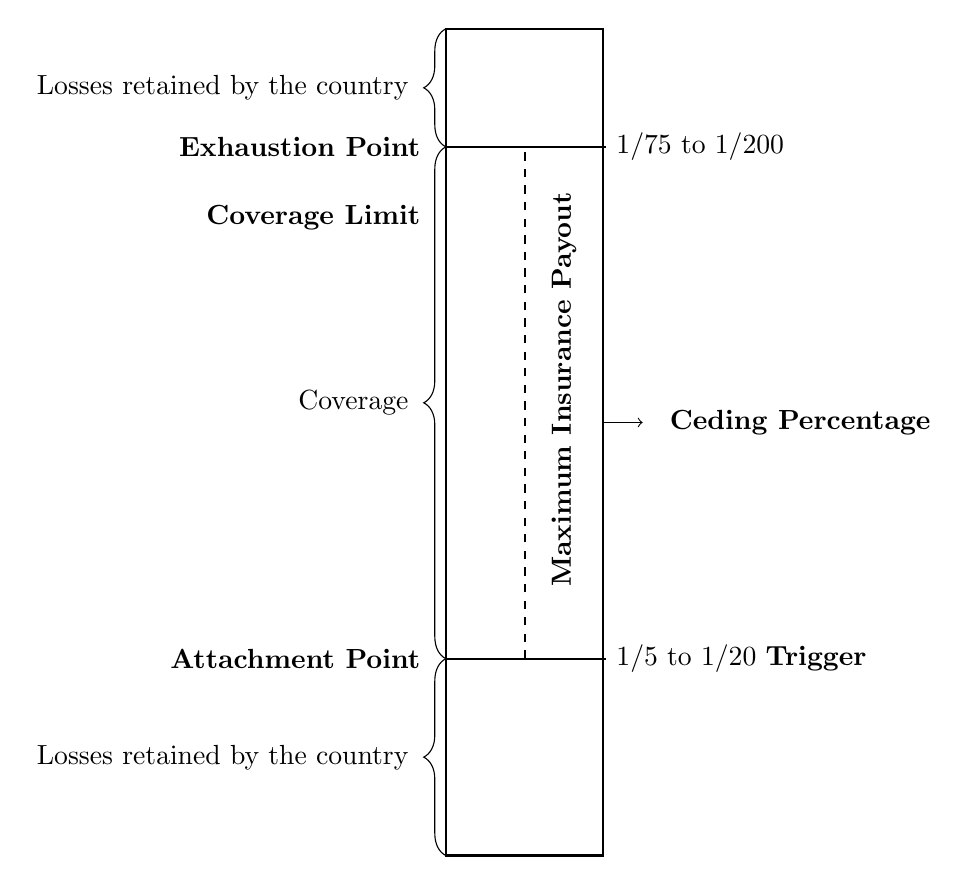
\begin{tikzpicture}

% Define dimensions
\def\barwidth{2cm}
\def\attachmentpoint{2.5cm}
\def\coverageheight{6cm}
\def\exhaustionheight{9cm}

% Draw main coverage bar
\draw[thick] (0,0) rectangle (\barwidth, \exhaustionheight + 1.5cm);
\draw[thick, dashed] (1,\attachmentpoint) -- (1, \exhaustionheight);

% Label sections on the left side
\node[anchor=east] at (-0.2, 0.9*\exhaustionheight) {\textbf{Coverage Limit}};
\node[anchor=east] at (-0.2, \exhaustionheight) {\textbf{Exhaustion Point}};
\node[anchor=east, rotate=90] at (1.5, 0.95*\exhaustionheight) {\textbf{Maximum Insurance Payout}};

% Draw braces and labels for bar sections
\draw[decorate, decoration={brace, mirror, amplitude=8pt}] (0, \attachmentpoint) -- (0, 0) node[midway, left, xshift=-10pt] {Losses retained by the country};
\draw[decorate, decoration={brace, mirror, amplitude=8pt}] (0, \exhaustionheight) -- (0, \attachmentpoint) node[midway, left, xshift=-10pt] {Coverage};
\draw[decorate, decoration={brace, amplitude=8pt}] (0, \exhaustionheight) -- (0, \exhaustionheight + 1.5cm) node[midway, left, xshift=-10pt] {Losses retained by the country};

% Draw right side labels for Ceding Percentage and Trigger

\draw[->] (\barwidth, \attachmentpoint + 0.5*\coverageheight) -- +(0.5cm, 0);
\node[align=left] at (4.5, \attachmentpoint + 0.5*\coverageheight) {\textbf{Ceding Percentage}};

% Add horizontal dashed lines
\node[anchor=east] at (-0.2, \attachmentpoint) {\textbf{Attachment Point}};
\draw[thick] (0, \attachmentpoint) -- (\barwidth + 1, \attachmentpoint) node[anchor=west] {1/5 to 1/20 \textbf{Trigger} };
\draw[thick] (0, \exhaustionheight) -- (\barwidth + 1, \exhaustionheight) node[anchor=west] {1/75 to 1/200};
\end{tikzpicture}
\end{adjustbox}
\subcaption{}
\label{fig:ins_module}
\end{subfigure}
\hspace{1cm}
\begin{subfigure}[b]{0.35\textwidth}
\begin{adjustbox}{width=\textwidth}
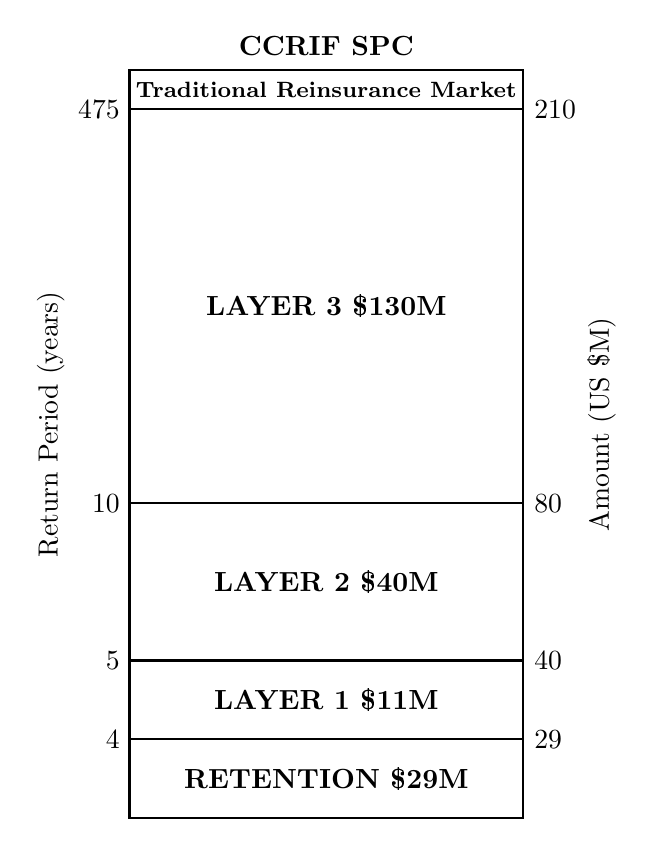
\begin{tikzpicture}

% Define the width of the blocks
\def\blockwidth{5cm}

% Draw CCRIF Retention block
\draw[thick] (0,0) rectangle (\blockwidth,1) node[midway] {\textbf{RETENTION \$29M}};
\node[anchor=east] at (0, 1) {4};
\node[anchor=west] at (\blockwidth + 0.5, 1) {29};

% Draw Layer 1 block
\draw[thick] (0,1) rectangle (\blockwidth,2) node[midway] {\textbf{LAYER 1 \$11M}};
\node[anchor=east] at (0, 2) {5};
\node[anchor=west] at (\blockwidth + 0.5, 2) {40};

% Draw Layer 2 block
\draw[thick] (0,2) rectangle (\blockwidth,4) node[midway] {\textbf{LAYER 2 \$40M}};
\node[anchor=east] at (0, 4) {10};
\node[anchor=west] at (\blockwidth + 0.5, 4) {80};

% Draw Layer 3 block
\draw[thick] (0,4) rectangle (\blockwidth,9) node[midway] {\textbf{LAYER 3 \$130M}};
\node[anchor=east] at (0, 9) {475};
\node[anchor=west] at (\blockwidth + 0.5, 9) {210};

% Draw Traditional Reinsurance Market label at the top
\draw[thick] (0,9) rectangle (\blockwidth,9.5) node[midway] {\footnotesize \textbf{Traditional Reinsurance Market}};

% Header and title
\node[align=center] at (2.5, 9.8) {\textbf{CCRIF SPC}};

% Labels for Return Period and Amount
\node[align=center, rotate=90] at (-1, 5) {Return Period (years)};
\node[align=center, rotate=90] at (6, 5) {Amount (US \$M)};

\end{tikzpicture}
\end{adjustbox}
\subcaption{}
\label{fig:rein_module}
\end{subfigure}
\label{fig:ccrif_module_program}
\end{figure}

CCRIF's insurance module is presented in 
Figure \ref{fig:ins_module} (\cite{CCRF_TC2023_2023}). Each country’s insurance policy parameters are carefully selected to provide optimal coverage that aligns with its risk management strategy while staying within budget. The trigger point range of 1/5 to 1/20 represents the likelihood or frequency threshold at which an insurance policy begins to pay out. The maximum payout a country can receive is determined by subtracting the attachment point from the exhaustion point and multiplying the result by the ceding percentage. The attachment point is the loss level at which the policy begins to pay out, while the exhaustion point represents the upper threshold beyond which no further payouts are made. The coverage limit, which is the highest dollar amount a policy can pay out, is based on the range between these two points and adjusted by the ceding percentage. The ceding percentage plays a crucial role in determining the premium. Once the attachment and exhaustion points are set, there is a direct relationship between the premium amount and the ceding percentage. A higher ceding percentage results in a higher premium, as it increases the portion of potential losses that can be covered. 

It is important to mention that CCRIF insurance exclusively covers government losses, which are calculated as a percentage of a country’s total national losses. This structure ensures that payouts are aligned with the financial impact on public sector infrastructure and services. It is therefore reasonable to assume that the payout for each country is analogous to its GDP, a method that we shall apply for calibrating the models' parameters. 

CCRIF retains US \$29.0 million for payouts and has secured an additional US \$181.0 million in reinsurance capacity above this retention to enhance its claims-paying capacity (\cite{CCRF_AnnualReport_2023}). This reinsurance structure, capped at US \$210.0 million, provides coverage for aggregate annual losses (as in our framework). This structure is illustrated in Figure \ref{fig:rein_module}.
% \begin{figure}[t]
% \centering
% \caption{Aggregate Excess of Loss Program 2022/2023 for Caribbean TC.
% % CCRIF retains US \$29 million, while Layers 1, 2, and 3, totaling US \$181 million, are covered by reinsurers.
% }
% \begin{tikzpicture}

% % Define dimensions
% \def\barwidth{2cm}
% \def\attachmentpoint{2.5cm}
% \def\coverageheight{6cm}
% \def\exhaustionheight{9cm}

% % Draw main coverage bar
% \draw[thick] (0,0) rectangle (\barwidth, \exhaustionheight + 1.5cm);
% \draw[thick, dashed] (1,\attachmentpoint) -- (1, \exhaustionheight);

% % Label sections on the left side
% \node[anchor=east] at (-0.2, 0.9*\exhaustionheight) {\textbf{Coverage Limit}};
% \node[anchor=east] at (-0.2, \exhaustionheight) {\textbf{Exhaustion Point}};
% \node[anchor=east, rotate=90] at (1.5, 0.95*\exhaustionheight) {\textbf{Maximum Insurance Payout}};

% % Draw braces and labels for bar sections
% \draw[decorate, decoration={brace, mirror, amplitude=8pt}] (0, \attachmentpoint) -- (0, 0) node[midway, left, xshift=-10pt] {Losses retained by the country};
% \draw[decorate, decoration={brace, mirror, amplitude=8pt}] (0, \exhaustionheight) -- (0, \attachmentpoint) node[midway, left, xshift=-10pt] {Coverage};
% \draw[decorate, decoration={brace, amplitude=8pt}] (0, \exhaustionheight) -- (0, \exhaustionheight + 1.5cm) node[midway, left, xshift=-10pt] {Losses retained by the country};

% % Draw right side labels for Ceding Percentage and Trigger

% \draw[->] (\barwidth, \attachmentpoint + 0.5*\coverageheight) -- +(0.5cm, 0);
% \node[align=left] at (4.5, \attachmentpoint + 0.5*\coverageheight) {\textbf{Ceding Percentage}};

% % Add horizontal dashed lines
% \node[anchor=east] at (-0.2, \attachmentpoint) {\textbf{Attachment Point}};
% \draw[thick] (0, \attachmentpoint) -- (\barwidth + 1, \attachmentpoint) node[anchor=west] {1/5 to 1/20 \textbf{Trigger} };
% \draw[thick] (0, \exhaustionheight) -- (\barwidth + 1, \exhaustionheight) node[anchor=west] {1/75 to 1/200};
% \end{tikzpicture}
% \label{fig:rein_module}
% \end{figure}

\subsection{Model Calibration}\label{app:ccrif_tc_year_info}
CCRIF uses a parametric insurance model that follows the same general structure across all member countries, but the parameters and triggers within that model can vary based on the individual contracts signed by each country. The parameters and thresholds (such as wind speed, rainfall intensity, or earthquake magnitude that trigger payouts) are customized based on each country’s risk profile and needs. Since this information is not publicly available, it is difficult to accurately estimate the actual losses based solely on their payout data. The model triggers payouts based on predefined parameters (such as wind speed or rainfall), rather than on detailed assessments of actual damage, making it challenging to directly correlate payouts with real losses. 
% Based on the data CCRIF's website (\cite{ccrif_payouts}), the payouts from 2007-2024 is given in Table \ref{tab:payout}.\footnote{Note, for example, Trinidad and Tobago is a twin-island state where they are treated as a single sovereign country. However, since CCRIF parametric insurance policies are often tailored to reflect the unique risk profiles of individual islands or regions within a country, the payout for each is calculated differently even if both islands are covered under the same policy. For example, if a hurricane primarily impacts Tobago but not Trinidad, the payout would be based on the parametric data for Tobago, even though the policy covers both islands.}
% \begin{table}[htp!]
%     \centering
%     \caption{Payouts by Country \& Organization. All amounts are in USD, rounded to the nearest integer.}
%     \begin{tabular}{lrrr}
% \toprule\toprule
%  & Mean & Variance & Occurrences \\
% Members &  &  &  \\
% \midrule
% Anguilla & 2404674 & 6528031084693 & 5 \\
% Antigua \& Barbuda & 3365315 & 6889360828127 & 3 \\
% Barbados & 2721767 & 7216082053012 & 8 \\
% Belize & 306403 & 11599983533 & 3 \\
% British Virgin Islands & 700836 & 22063685982 & 2 \\
% Cayman Turtle Conservation and Education Centre & 119474 & 0 & 1 \\
% Dominica & 5819749 & 60992875234082 & 4 \\
% Grenada & 11113147 & 255118062762243 & 5 \\
% Guatemala & 5002098 & 1888110961310 & 2 \\
% Haiti & 15655929 & 181392406532855 & 5 \\
% Jamaica & 10029313 & 27376980466945 & 3 \\
% Nicaragua & 6862580 & 43949336827420 & 6 \\
% Panama & 2670556 & 0 & 1 \\
% Saint Lucia & 2028348 & 2244750082608 & 4 \\
% St. Kitts \& Nevis & 1619938 & 261998827027 & 3 \\
% St. Vincent \& the Grenadines & 871430 & 440924300764 & 4 \\
% The Bahamas & 4329250 & 26118987774803 & 3 \\
% Tobago & 409703 & 39682834733 & 4 \\
% Trinidad & 3687936 & 4266526338818 & 5 \\
% Turks \& Caicos Islands & 5396980 & 27688273270975 & 4 \\
% \bottomrule\bottomrule
% \end{tabular}
%     \label{tab:payout}
% \end{table}
% In Figure \ref{fig:mean_payout} and Figure \ref{fig:var_payout}, the mean and variance which we are going to use in our model is presented. 

The yearly payout data is considered as loss data, which is divided by 100,000 for the following calculations. For each year the realization of the sum of losses is denoted by $S_{n,year}=\sum_{i=1}^nX_{i,year},$ where $X_{i,year}$ is the individual loss for country $i$ in any year of the data. In order to estimate the annual risk variance for each country, we first estimate the mean and the variance of the aggregate annual losses $(m_n,s_n^2).$ The parameters of $m_n$ and $s_n^2$ are found through the maximum likelihood estimate. The maximum likelihood estimate (M USD) is given by 
\[
\hat{m}_n = \frac{1}{n} \sum_{year}^{} S_{n,year}\approx 159.56,\quad \hat{s}^2_n = \frac{1}{\#year} \sum_{year}^{} (S_{n,year} - \hat{m}_n)^2\approx56,598.28
\]
Based on this, we find the mean and the variance of each country $j$ using the following approximation:
    {
\begin{align*}
\text{Adjusted\_Variance}_i =\hat{\sigma}_i^2:= k^2 \times \left(\text{Occurrence\_Probability}_i\right)\times \left(1-\text{Occurrence\_Probability}_i\right) \times \left(\text{GDP}_i\right)^2
\end{align*}
}
where $k$ is the constant to match the sum of adjusted variances to the variance of total loss, under the assumption that we have the constant correlation $\rho=0.3$ among any pair of two countries, {\it i.e.,} 
\[ \sum_{j}\hat{\sigma}_j^2+2\rho\sum_{i\neq j}\hat{\sigma}_i\hat{\sigma}_j= \hat{s}_n^2
\]
Then,     {$k\approx 0.000386.$} Based on this, the adjusted variance can be computed, which is presented in Table \ref{tab:summary_country}.
\begin{table}[t]
\caption{    {Summary Table for each member.}}
\centering
\resizebox{\linewidth}{!}{%
\begin{tabular}{lrrrrr}
\toprule\toprule
Members & Year & GDP (\$M USD) & Occurrence Probability & Adjusted Variance\\
\midrule
Anguilla & 2007 & 452 & 0.0727 & 0.016 \\
Antigua \& Barbuda & 2007 & 2,030 & 0.0364 & 0.081 \\
Barbados & 2007 & 6,390 & 0.1091 & 7.254 \\
Belize & 2007 & 3,280 & 0.0545 & 0.478 \\
Cayman Islands & 2007 & 6,990 & 0.0182 & 0.241 \\
Dominica & 2007 & 654 & 0.0364 & 0.008 \\
Grenada & 2007 & 1,320 & 0.0910 & 0.215 \\
Haiti & 2007 & 14,340 & 0.0545 & 9.133 \\
Jamaica & 2007 & 32,420 & 0.0545 & 46.680 \\
Saint Lucia & 2007 & 2,520 & 0.0545 & 0.282 \\
St. Kitts \& Nevis & 2007 & 1,080 & 0.0364 & 0.023 \\
St. Vincent \& the Grenadines & 2007 & 1,070 & 0.0727 & 2.90 \\
The Bahamas & 2007 & 14,340 & 0.0545 & 0.090 \\
The Republic of Trinidad and Tobago & 2007 & 28,140 & 0.0364 & 15.630 \\
Turks \& Caicos Islands & 2007 & 1,400 & 0.0727 & 0.155 \\
Nicaragua & 2015 & 14,340 & 0.0910 & 25.369 \\
British Virgin Islands & 2018 & 476 & 0.0182 & 0.001 \\
Panama & 2018 & 83,380 & 0.0182 & 34.307 \\
Guatemala & 2019 & 247,610 & 0.0182 & 302.549 \\
\bottomrule\bottomrule
\end{tabular}
}
\noindent\begin{minipage}{\textwidth}
\raggedright
%\NOTE{{\it Note}: The adjusted means are omitted since they can be computed by taking the square root of the adjusted variances.}
\end{minipage}
\label{tab:summary_country}
\end{table}
% \begin{table}[t]
% \caption{Summary Table for each member.}
% \centering
% \resizebox{\linewidth}{!}{%
% \begin{tabular}{lrrrrr}
% \toprule\toprule
% Members & Year & GDP (\$M USD) & Occurrence Probability & Adjusted Variance\\
% \midrule
% Anguilla & 2007 & 452 & 0.0727 & 0.52 \\
% Antigua \& Barbuda & 2007 & 2,030 & 0.0364 & 2.61 \\
% Barbados & 2007 & 6,390 & 0.1091 & 232.73 \\
% Belize & 2007 & 3,280 & 0.0545 & 15.33 \\
% Cayman Islands & 2007 & 6,990 & 0.0182 & 7.74 \\
% Dominica & 2007 & 654 & 0.0364 & 0.27 \\
% Grenada & 2007 & 1,320 & 0.0910 & 6.90 \\
% Haiti & 2007 & 14,340 & 0.0545 & 293.01 \\
% Jamaica & 2007 & 32,420 & 0.0545 & 1,497.66 \\
% Saint Lucia & 2007 & 2,520 & 0.0545 & 9.05 \\
% St. Kitts \& Nevis & 2007 & 1,080 & 0.0364 & 0.74 \\
% St. Vincent \& the Grenadines & 2007 & 1,070 & 0.0727 & 2.90 \\
% The Bahamas & 2007 & 14,340 & 0.0545 & 293.01 \\
% The Republic of Trinidad and Tobago & 2007 & 28,140 & 0.0364 & 501.48 \\
% Turks \& Caicos Islands & 2007 & 1,400 & 0.0727 & 4.96 \\
% Nicaragua & 2015 & 14,340 & 0.0910 & 813.92 \\
% British Virgin Islands & 2018 & 476 & 0.0182 & 0.04 \\
% Panama & 2018 & 83,380 & 0.0182 & 1,100.70 \\
% Guatemala & 2019 & 247,610 & 0.0182 & 9,706.92 \\
% \bottomrule\bottomrule
% \end{tabular}
% }
% \noindent\begin{minipage}{\textwidth}
% \raggedright
% %\NOTE{{\it Note}: The adjusted means are omitted since they can be computed by taking the square root of the adjusted variances.}
% \end{minipage}
% \label{tab:summary_country}
% \end{table}
% \begin{figure}[htp!]
%     \centering
%     \includegraphics[width=0.7\linewidth]{Figures/TC_Mean.png}
%     \caption{Summary Table for each country.}
%     \label{fig:summary_country}
% \end{figure}

Given Table \ref{tab:summary_country}, by approximating the payouts as the actual losses, we can apply our model to evaluate the potential impact of a new candidate joining in the following year. For the implementation, we need to estimate two key parameters: (1) risk tolerance coefficients, and (2) correlation coefficients among countries' risks. To simplify the analysis, it is assumed that all countries have the same pairwise correlation $\rho=0.3$, and the same risk tolerance level $\delta=1$. Note that higher correlations are expected among some countries that frequently experience losses from same disasters.

Following its history, the existing pool consists of the following 16 founding members- Dominica, Saint Lucia, Turks \& Caicos Islands, Haiti, Anguilla, Barbados, St. Vincent \& the Grenadines, St. Kitts \& Nevis, Belize, Antigua \& Barbuda, The Bahamas, The Republic of Trinidad and Tobago, Jamaica, Grenada, Cayman Islands. We consider the joining of other members- British Virgin Islands, Nicaragua, Panama, and Guatemala. The evolution of membership is summarized in Table \ref{tab:summary_country} (\cite{ccrif_members}, \cite{caricom_ccrif}, \cite{worldbank_ccrif}, \cite{ccrif_carec_webinar}, and \cite{ccrif_honduras}).
% \begin{table}[t]
% \centering
% \caption{CCRIF Membership Evolution by Year from 2007 to 2023}
% \begin{adjustbox}{width=\textwidth}
% \begin{tabular}{rc}
% \toprule\toprule
% Year &                                            Members \\
% \midrule
% \multirow{3}{*}{2007} & Anguilla, Antigua and Barbuda, The Bahamas, Barbados, Belize, Bermuda, Cayman Islands,\\
% &   Dominica, Grenada, Haiti, Jamaica, Saint Kitts and Nevis, Saint Lucia,\\
% &Saint Vincent and the Grenadines, The Republic of Trinidad and Tobago, The Turks and Caicos Islands \\
% 2015 &   Nicaragua \\
% 2018 &  British Virgin Islands, Montserrat, Sint Maarten, Panama \\
% 2019 &  Guatemala  \\
% 2023 & Honduras\\
% \bottomrule\bottomrule
% \end{tabular}
% \end{adjustbox}
% \label{app:tab:evolution}
% \end{table}

\subsection{Results}
As described in the paper, the expansion process is considered one candidate at a time. A candidate may represent a single country or a region consisting of multiple countries. To simplify the analysis, we initially focus on the expansion involving a single country. The simulation results are shown in Figures \ref{fig:ccrif_fair} and \ref{fig:CCRIF_equi}, and the summary of expansion is presented in Table \ref{app:tab:CCRIF_summary}. 

The model suggests that it might not always be advantageous to incorporate new members. The addition of members with high variance, such as Guatemala, Nicaragua, and Panama—each exhibiting significantly higher variances than the existing pool—could have an adverse impact on the pool under risk-conservative pricing rules like Fairness Principle (Figure \ref{fig:ccrif_fair_wo_rein}). In Figure \ref{fig:ccrif_fair_w_rein}, this holds true regardless of whether reinsurance is in place. Conversely, if members' decisions are made based on risk-seeking pricing rules like Equilibrium Principle, the British Virgin Islands    {, Nicaragua, and Panama} would be unsuitable for inclusion due to its low risk profile (Figure \ref{fig:CCRIF_equi_wo}). In Figure \ref{fig:CCRIF_equi_w}, under the stricter acceptance criteria with reinsurance,     {even Guatemala is not accepted}. In this context, the pool favors candidates seeking to offload risks rather than those inclined to assume additional risks.

\begin{figure}[t]
\centering
\caption{CCRIF: Expansion under Fairness Principle without and with reinsurance.}
\begin{subfigure}[b]{0.48\textwidth}
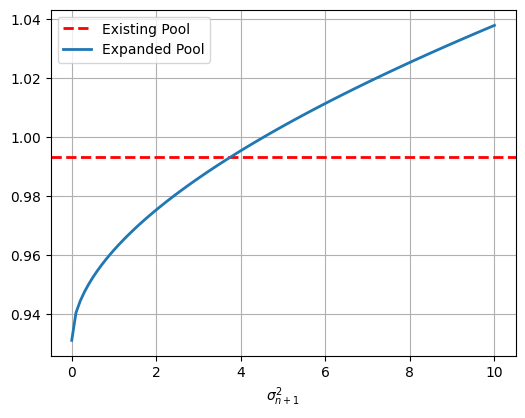
\includegraphics[width=\linewidth]{Figures/indicator_FP_wo.png}
\subcaption{Without reinsurance}
\label{fig:ccrif_fair_wo_rein}
\end{subfigure}
\hfill
\begin{subfigure}[b]{0.48\textwidth}
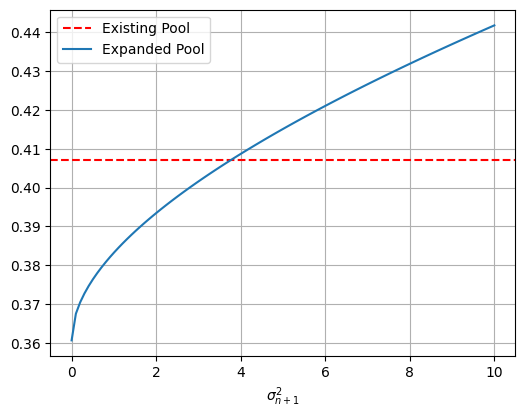
\includegraphics[width=\linewidth]{Figures/indicator_FP_w.png}
\subcaption{With reinsurance}
\label{fig:ccrif_fair_w_rein}
\end{subfigure}
\label{fig:ccrif_fair}
\vspace{0pt} 
\noindent\begin{minipage}{\textwidth}
\raggedright
\NOTE{{\it Note}: On the left panel, the deviation-tolerance ratios are shown, while the values of $l$ function \eqref{eq:rein_strong} from the main text are presented on the right panel. In both cases, the existing members benefit from the expansion when blue lines are below red lines.}
\end{minipage}
\end{figure}



\begin{figure}[t]
\centering
\caption{CCRIF: Expansion under Equilibrium Principle without and with reinsurance.}
\begin{subfigure}[b]{0.8\textwidth}
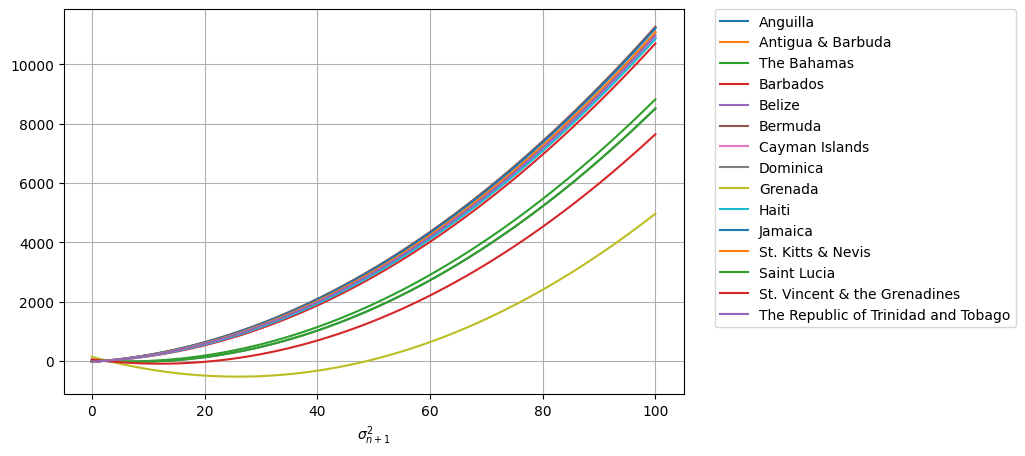
\includegraphics[width=\linewidth]{Figures/indicator_EP_wo.png}
\subcaption{Without reinsurance}
\label{fig:CCRIF_equi_wo}
\end{subfigure}

\begin{subfigure}[b]{0.8\textwidth}
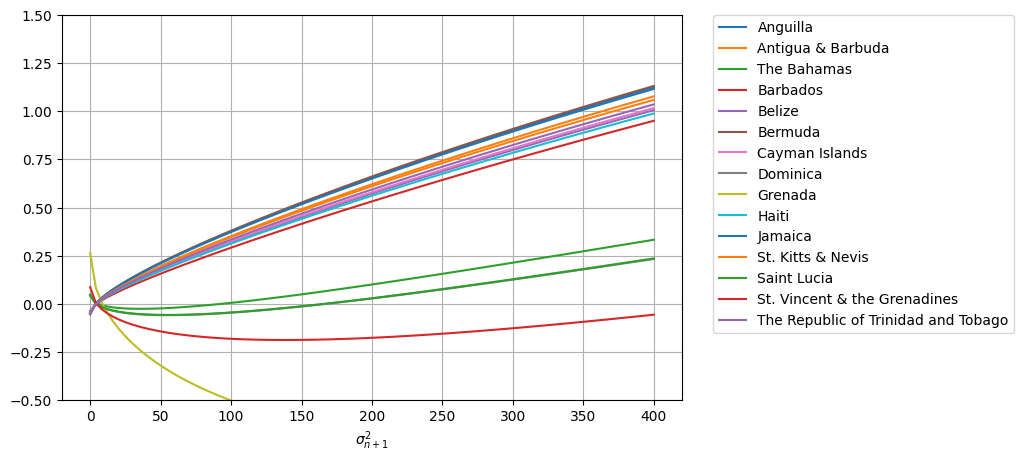
\includegraphics[width=\linewidth]{Figures/indicator_EP_w.png}
\subcaption{With reinsurance}
\label{fig:CCRIF_equi_w}
\end{subfigure}
\label{fig:CCRIF_equi}
\noindent\begin{minipage}{\textwidth}
\raggedright
\NOTE{{\it Note}: On the top panel, the values of $f$ function \eqref{eq:withsamecor} from the main text are presented, while the results of Monte-Carlo simulations for the difference in entropic risk measures are presented on the bottom panel. In both cases, each member in the existing pool benefits from the expansion when the graph is above zero.}
\end{minipage}
\end{figure}

\begin{table}[t]
\centering
\caption{    {CCRIF: Summary of Expansion (checkmark means SC)}}
\begin{adjustbox}{width=0.7\textwidth}
\begin{tabular}{l|cc|cccc|cccc}
\hline\hline
\multirow{3}{*}{}      & \multicolumn{2}{c|}{\multirow{2}{*}{DTR}} & \multicolumn{4}{c|}{W/O Reinsurance}    & \multicolumn{4}{c}{W/ Reinsurance} \\ 

\cline{4-11} 
& \multicolumn{2}{c|}{}  & \multicolumn{2}{c|}{FP} & \multicolumn{2}{c|}{EP}    & \multicolumn{2}{c|}{FP} & \multicolumn{2}{c}{EP}      \\ 

\cline{1-11} pairwise correlation 
& \multicolumn{1}{c|}{0.1}      & 0.3& \multicolumn{1}{c|}{0.1}    & \multicolumn{1}{c|}{0.3}    & \multicolumn{1}{c|}{0.1}    & 0.3    & \multicolumn{1}{c|}{0.1}    & \multicolumn{1}{c|}{0.3}    & \multicolumn{1}{c|}{0.1}    & 0.3 \\ 

\hline\hline
Existing Pool   & \multicolumn{1}{c|}{1.02}  & 0.99      & \multicolumn{1}{c|}{-} & \multicolumn{1}{c|}{-} & \multicolumn{1}{c|}{-} & - & \multicolumn{1}{c|}{-} & \multicolumn{1}{c|}{-} & \multicolumn{1}{c|}{-} & -   \\ \hline

British Virgin Islands & \multicolumn{1}{c|}{0.04}  & 0.03      & \multicolumn{1}{c|}{\checkmark} & \multicolumn{1}{c|}{\checkmark} & \multicolumn{1}{c|}{}  &   & \multicolumn{1}{c|}{\checkmark} & \multicolumn{1}{c|}{\checkmark} & \multicolumn{1}{c|}{}  &     \\ \hline

Guatemala  & \multicolumn{1}{c|}{23.04}  & 17.39     & \multicolumn{1}{c|}{}  & \multicolumn{1}{c|}{}  & \multicolumn{1}{c|}{\checkmark} & \checkmark & \multicolumn{1}{c|}{}  & \multicolumn{1}{c|}{}  & \multicolumn{1}{c|}{\checkmark} &     \\ \hline

Nicaragua  & \multicolumn{1}{c|}{6.67}  & 5.03      & \multicolumn{1}{c|}{}  & \multicolumn{1}{c|}{}  & \multicolumn{1}{c|}{\checkmark} &   & \multicolumn{1}{c|}{}  & \multicolumn{1}{c|}{}  & \multicolumn{1}{c|}{\checkmark} &     \\ \hline

Panama     & \multicolumn{1}{c|}{7.76}  & 5.85      & \multicolumn{1}{c|}{}  & \multicolumn{1}{c|}{}  & \multicolumn{1}{c|}{\checkmark} &   & \multicolumn{1}{c|}{}  & \multicolumn{1}{c|}{}  & \multicolumn{1}{c|}{\checkmark} &     \\ \hline\hline
\end{tabular}
\end{adjustbox}
\label{app:tab:CCRIF_summary}
\end{table}

\section{Potential Healthcare Sharing in China}\label{app:health}
This example explores the application of fairness and equilibrium principles with and without reinsurance, using health insurance data in China. The first section provides an overview of the data used in the analysis, and the second section explains the design of the simulation setup. The key findings of the analysis are summarized in the result section. It highlights how the conditions for expanding risk pools vary under the fairness and equilibrium principles, both with and without reinsurance, providing critical insights into the practical implications of each framework.

\subsection{Data}\label{app:health_data}
The data is collected, pertaining to healthcare services and insurance claims in the year of 2020 within the framework of China's health insurance system. The dataset provides a range of information that includes demographic details, healthcare service utilization, and financial compensation for medical treatments. Specifically, the data includes the following attributes:
\begin{enumerate}
\item Demographic Information: Gender and date of birth. The birth date specifies the age of the individuals at the time of the claim, which can be used to infer age.
\item Healthcare Service Details: The names of hospitals visited are listed, along with the corresponding regions or districts in China.
\item Medical Condition: The specific medical condition or diagnosis for which the individual sought treatment is identified.
\item Financial Information: The amount of financial reimbursement or coverage provided under the insurance claim, denoted in yuan.
\end{enumerate}
The example data is given in Table \ref{tab:sample_data}.
\begin{table}[t]
\centering
\caption{Sample Data}
\resizebox{\linewidth}{!}{%
\begin{tabular}{llll}
\toprule\toprule
Category & First person & Second person & Third person \\
\midrule
Gender & M & F & F \\
Date of Birth & 1981-03-17 & 1987-07-31 & 1978-09-30 \\
Hospital Visited & Luodian Hospital, Baoshan District, Shanghai & Beijing Longxi Hospital & Shenzhen Longhua District Maternal and Child Health Hospital \\
Disease Name & Lower limb fracture & Thyroid Nodules & Missed abortion \\
Compensation Amount & 198.00 & 185.94 & 9.90 \\
\bottomrule\bottomrule
\end{tabular}
}    
\label{tab:sample_data}
\end{table}

\subsection{Model Calibration}\label{app:health_simul}
The data was organized by extracting regional information based on the hospitals visited by individuals for their medical treatment. The hospital names in the dataset either explicitly mentioned the name of the region, or provided enough contextual clues to infer the region. 

After determining the region for each claim, the data was grouped accordingly. This grouping allowed us to find the estimates for the parameters of distributions across different areas. To standardize the compensation amounts for easier simulation, the original values were divided by 100. Then, for each region, we calculated the number of claims, the average mean compensation, and the variance of the compensation amounts. These estimations are listed in Table \ref{tab:region_summary}. 

We selected regions with a sufficiently large number of claims and ensured that the chosen cities have comparable size. A common pairwise correlation of 0.3 and a common risk tolerance equal to 1 for all cities are assumed.

\begin{table}[t]
\centering
\caption{Mean and variance of compensation for each region}
\begin{tabular}{lrrr}
\toprule\toprule
Region & Count & Mean & Variance \\
\midrule
Beijing & 4,357 & 1.78 & 11.90 \\
Chengdu & 312 & 0.88 & 3.67 \\
Chongqing & 400 & 1.40 & 9.68 \\
Dalian & 450 & 2.34 & 30.90 \\
Guangzhou & 223 & 2.40 & 31.81 \\
Hangzhou & 116 & 1.45 & 22.55 \\
Nanjing & 1,096 & 1.29 & 12.88 \\
Qingdao & 172 & 1.29 & 9.86 \\
Shanghai & 11,107 & 1.35 & 9.16 \\
Shenyang & 119 & 2.17 & 14.01 \\
Shenzhen & 233 & 1.69 & 9.67 \\
Suzhou & 214 & 1.29 & 19.56 \\
Tianjin & 1,211 & 1.06 & 15.57 \\
\bottomrule\bottomrule
\end{tabular}
\label{tab:region_summary}
\end{table}

To construct the case study following our framework, we need to impose an existing group of cities. For this, we consider a reasonable formation of geographic criterion and let major cities of northeastern China, such as Beijing, Tianjin, Shenyang, and Dalian as the existing agents. We then examine the expansion of this pool for a number of different candidates (e.g. other Eastern Coastal cities such as Shanghai, Nanjing, Suzhou, and Hangzhou, or Southern Chinese cities like Shenzhen and Guangzhou). 

\subsection{Results}
As outlined in the paper, the expansion considers one candidate, which could be a single city or a region comprising multiple cities. We work on the simplified case of single city expansion (where the reinsurance level $\beta$ is set equal to 1.64).

The FP dictates that the expansion will be accepted in SC sense if the variance of the candidate city is less than 25, regardless of the presence of reinsurance (Figures \ref{app:fig:china_fair_wo} and \ref{app:fig:china_fair_w}). Based on this criterion, the existing pool agrees to include all candidate cities except Guangzhou (whose risk's variance is rather high). In contrast, under EP, the acceptance threshold varies depending on whether reinsurance is applied. Without reinsurance, EP allows expansion to candidates with variances larger than 3.5, meaning that all cities are accepted (Figure \ref{app:fig:china_equi_wo}). However, with reinsurance, the threshold rises to 11.2, resulting in the exclusion of cities such as Chengdu (Figure \ref{app:fig:china_equi_w}). The results are summarized in Table \ref{app:tab:expansion_insu} and Figure \ref{app:fig:china}.
\begin{table}[t]
\centering
\caption{Summary of statistics and decision-making for the expansion of health-share}
\begin{adjustbox}{width=0.6\textwidth}
\begin{tabular}{l|c|cc|cc}
\hline\hline
&  & \multicolumn{2}{c|}{W/O Reinsurance}  & \multicolumn{2}{c|}{W/ Reinsurance} \\ \hline
& D/T & \multicolumn{1}{c|}{Fairness}  & Equilibrium & \multicolumn{1}{c|}{Fairness}  & Equilibrium \\ \hline\hline
Existing pool &    2.9 & \multicolumn{1}{c|}{-} & - & \multicolumn{1}{c|}{-} & - \\ \hline
Guangzhou&    5.64 & \multicolumn{1}{c|}{}  & \checkmark & \multicolumn{1}{c|}{}  & \checkmark \\ \hline
Chengdu  &   1.92  & \multicolumn{1}{c|}{\checkmark} & \multicolumn{1}{c|}{\checkmark}  & \multicolumn{1}{c|}{\checkmark} &   \\ \hline
Chongqing&   3.11  & \multicolumn{1}{c|}{\checkmark} & \multicolumn{1}{c|}{\checkmark}  & \multicolumn{1}{c|}{\checkmark} &  \\ \hline
Qingdao  &   3.14  & \multicolumn{1}{c|}{\checkmark} & \multicolumn{1}{c|}{\checkmark}  & \multicolumn{1}{c|}{\checkmark} &  \\ \hline
Shanghai &   3.03  & \multicolumn{1}{c|}{\checkmark} & \multicolumn{1}{c|}{\checkmark}  & \multicolumn{1}{c|}{\checkmark} &  \\ \hline
Shenzhen &    3.11 & \multicolumn{1}{c|}{\checkmark} & \multicolumn{1}{c|}{\checkmark}  & \multicolumn{1}{c|}{\checkmark} &   \\ \hline
Others   & -    & \multicolumn{1}{c|}{\checkmark} & \checkmark & \multicolumn{1}{c|}{\checkmark} & \checkmark \\ \hline\hline
\end{tabular}
\end{adjustbox}
\label{app:tab:expansion_insu}
\end{table}
\begin{figure}[t]
\centering
\caption{Strong Consensus under Fairness and Equilibrium Principle with and without reinsurance.}
\begin{subfigure}[b]{0.48\textwidth}
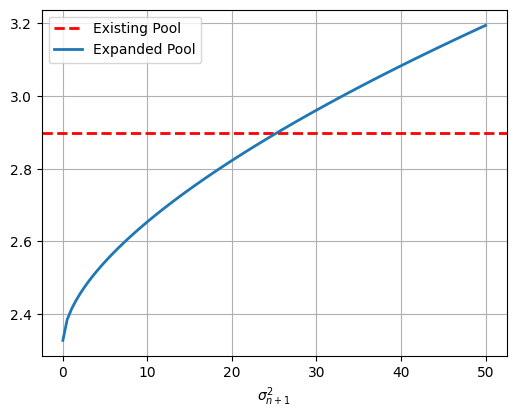
\includegraphics[width=\linewidth]{Figures/fair_region.png}
\subcaption{Fairness Principle without reinsurance}
\label{app:fig:china_fair_wo}
\end{subfigure}
\hfill
\begin{subfigure}[b]{0.48\textwidth}
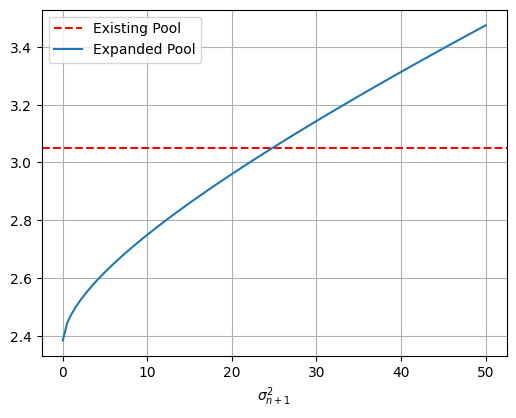
\includegraphics[width=\linewidth]{Figures/fair_region_rein.png}
\subcaption{Fairness Principle with reinsurance}
\label{app:fig:china_fair_w}
\end{subfigure}

\begin{subfigure}[b]{0.48\textwidth}
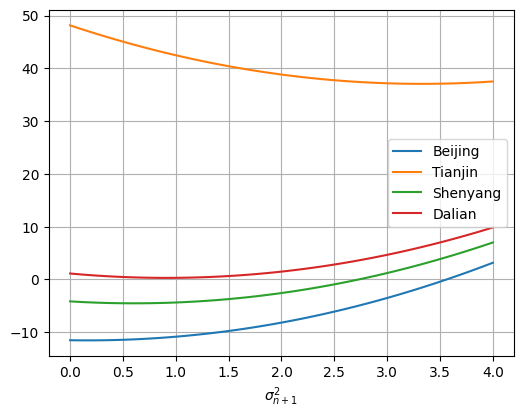
\includegraphics[width=\linewidth]{Figures/equi_region.png}
\subcaption{Equilibrium Principle without reinsurance}
\label{app:fig:china_equi_wo}
\end{subfigure}
\hfill
\begin{subfigure}[b]{0.48\textwidth}
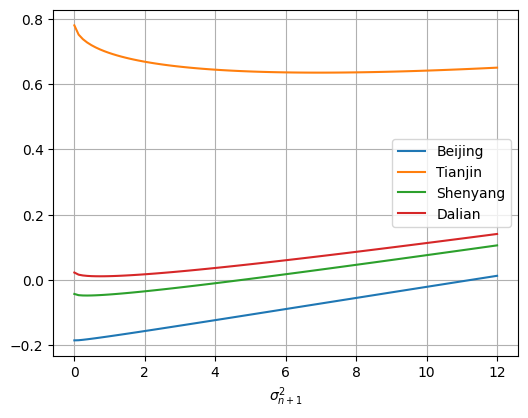
\includegraphics[width=\linewidth]{Figures/equi_region_rein.png}
\subcaption{Equilibrium Principle with reinsurance}
\label{app:fig:china_equi_w}
\end{subfigure}
\label{app:fig:china}
\noindent\begin{minipage}{\textwidth}
\raggedright
\NOTE{{\it Note}: On the top-left panel, the deviation-tolerance ratios shown, while the values of $l$ function \eqref{eq:rein_strong} from the main text are presented on the top-right panel. In both cases, the existing members benefit from the expansion when the blue line is below the red line. On the bottom-left panel, the values of $f$ function \eqref{eq:withsamecor} from the main text are presented, while the results of Monte-Carlo simulations for the difference in entropic risk measures are presented on the bottom-right panel. In both cases, each member in the existing pool benefits from the expansion when the graph is above zero.}
\end{minipage}
\end{figure}


These results align with the expectations outlined in the paper and highlight the fundamental differences between the fairness principle and the equilibrium principle in evaluating risk pool expansions. Under the fairness principle, lower-risk candidates are naturally favored because the fairness principle only charges premiums based on expected losses, which does not incorporate the additional compensation that higher-variance candidates could bring to the pool. Consequently, the fairness principle results in the acceptance of lower-risk candidates and excludes those exceeding the variance threshold, as seen in the rejection of Guangzhou. This preference remains unchanged regardless of whether reinsurance is applied, as the premium structure under fairness remains tied solely to the expectation of losses.

In contrast, the equilibrium principle reflects a preference for higher-risk candidates due to its pricing mechanism, which charges premiums based on variance. Candidates with higher variance are more attractive as they generate greater compensation for the existing members. Therefore, under the equilibrium principle without reinsurance, candidates with high variance are always preferred, as their higher risk translates into higher premiums that benefit the pool.

With the introduction of reinsurance under the equilibrium principle, the pool becomes less likely to accept candidates due to the competition between existing members and the reinsurer: the premiums are now partially transferred to the reinsurer. This reduces the incentive for the existing pool members to accept candidates, as the additional compensation from high risks is no longer fully retained within the pool. As a result, the equilibrium principle with reinsurance imposes a stricter acceptance threshold, excluding cities such as Chengdu, whereas without reinsurance, all candidates were accepted.

In summary, the results from two previous examples align with the theoretical expectations outlined in the paper, highlighting the distinct evaluation criteria of the two principles and the influence of reinsurance on the decision-making process. These findings also indirectly demonstrate why, in certain scenarios, the equilibrium principle can yield outcomes that are more beneficial from a societal perspective than the fairness principle. For instance, in situations where the existing pool possesses substantial wealth and is willing to take higher risks for greater premiums, the equilibrium principle can produce more favorable results compared to the fairness principle.

\section{Deviation of Normality Assumption}\label{app:simulation}
Our main analysis could be developed and studied under different probability distributions. Although it would be infeasible to have analytic conditions for weak and strong consensus, our setting provides all the necessary steps to simulate the conditions for both consensuses.

Of course, imposing other types of common risks' distributions, (such as  Exponential, Pareto, and Gamma), will not produce the exact same conditions as in the case of the normal distribution. However, we could examine whether the choice of other distributions will give similar \textit{qualitative} results. In other words, while the exact consensus conditions will not hold, we may get the same economic messages regarding, for instant, the effect of different pricing rules to acceptance of riskier candidates, the effect of higher risk correlations etc.

In order to examine the above, we have conducted a number of simulations in the view of our main results, under different common risk distributions and below we state a summary of the main outcomes. In short, we verify that even under heavy-tailed distributions our qualitative messages remain untouched.

More precisely, a central implication of this analysis is that risk pools tend to exhibit conservative behavior under the fairness principle, admitting only low-risk candidate. In contrast, under the equilibrium principle, existing members demonstrate a preference for high-risk candidates, as higher premiums offset the additional risk. This difference arises from the nature of the two pricing principles: while the fairness principle determines premiums based solely on the expected value of risk, the equilibrium principle incorporates also the second moment. Our simulation aims to examine whether this implication holds for other well-used distributions. We also could verify that higher correlation means that consensus conditions get stricter (since the diversification effect gets weaker).

We have run several Monte-Carlo simulations, considering a wide range of different parametrizations for Exponential, Pareto and Gamma distribution. Through this exercise we did verify our main qualitative results. In Section \ref{app:simul_result}- we give some indicative examples of these simulations.

\subsection{Simulation of Risk Measures under Different Distributions}
Suppose as in the main text that there are $n$ agents in an existing risk-sharing pool. The random vector $\mathbf{X}=(X_i)_{i\leq n}$ denotes the risk allocation before the risk sharing  (all realized at a terminal time), and $\mathbf{Y}^{(n)}=(Y_i^{(n)})_{i\leq n}$ stands for the risk allocation after the sharing, where the superscript $(n)$ is used to indicate the size of the risk pool. Recall that the entropic risk measure of agent $i$, is a map  $\rho_i$ defined as 
\begin{equation*}
\rho_i[X]=\CE_i[X]:=\delta_i\log\mathbb{E}[e^{\frac{1}{\delta_i}X}],
\end{equation*}
where $\delta_i>0$ is the risk tolerance of agent $i$, while for future reference we define $\Delta_n=\sum_{i=1}^n\delta_i$ as the aggregate risk tolerance of the existing ($n$-populated) group of agents. It is a well-known result that under cash-invariant risk measures Pareto-optimal allocations of $X$ are determined by the following problem 
\begin{equation}\label{app:eq:sharingproblem}
\min\left\{\sum_{i=1}^n\rho_i[Y_i^{(n)}]\right\},
\end{equation}
subject to the loss conservation condition $\sum_{i=1}^n X_i=\sum_{i=1}^n Y_i^{(n)}.$ Define the relative risk tolerance $\lambda_{n,i}:=\delta_i/\Delta_n$ and the aggregate risk $S_n:=\sum_{i=1}^n X_i.$ As mentioned before (see e.g. \cite{barrieu2005inf}), the linear risk-sharing rule is indeed the optimal even when the risks are not jointly normal. On the other hand, for the distributions whose moment-generating functions are not well-defined, the linear sharing could be considered as a meaningful ``sub-optimal'' sharing among agents in an approximating sense. Such sharing rule is given by
\begin{equation}
\mathbf{Y}^{(n)}=\mathbf{A}\mathbf{X}+\mathbf{p}^{(n)},
\end{equation}
where $\mathbf{A}=(a_{i,j})_{i,j=1,...,n}$ such that $a_{i,j}=\lambda_{n,i}$ for all $i,j=1,...,n$. The internal transfer $\mathbf{p}^{(n)}=(p_{n,i})_{i\leq n}$ within the group of $n$ agents is $n$-dimensional vector that is fixed by the pricing rule such as fairness principle and equilibrium principle. In the following simulations, the expansion under the strong consensus is considered, especially from the perspective of existing members, which must satisfy
\begin{equation}
\rho_i(Y_i^{(n)})\geq \rho_i(Y_i^{(n+1)}),\,  \forall i=1,2,...,n.
\end{equation}

Note again that the simulation conducted in this section is an approximation. For a finite sample size, the moment-generating function of Pareto distribution is finite because the extreme tail values are underestimated in the simulation process. The moment-generating function, which theoretically diverges to infinity for any positive \( t > 0 \), is computed as a sample-based approximation: $\mathbb{E}[e^{tX}] \approx \frac{1}{N} \sum_{i=1}^N e^{tX_i}.$ With a limited number of samples, it remains finite as the rare extreme tail events that dominate the divergence are unlikely to occur. However, as the sample size increases, the likelihood of including these extreme values grows, and the sample approximation begins to reflect the heavy-tailed nature of the Pareto distribution. In the limit as the sample size approaches infinity, the moment-generating function diverges, aligning with its theoretical behavior.

While the theoretical divergence of the moment-generating function is a characteristic of the Pareto distribution, the approximated results obtained through finite sample simulations are sufficient for our demonstration. The purpose of this simulation is to provide a consensus condition under other distributions than normal distributions. These approximations capture the key features of the Pareto distribution, including its heavy-tailed nature, without requiring an infinite number of samples. The results still allow us to analyze the impact of extreme values on risk measures,  enabling us to demonstrate the consensus condition under the Pareto distribution. In the same manner, the correlated exponential and Gamma distributions have a finite moment generating function for a finite sample size which is again enough for the demonstration in this section.

\begin{figure}[t]
\caption{Finite sample approximations of risk measures for the existing and expanded pools, based on the exponential distribution, under the fairness and equilibrium principles with varying values of $\lambda_3.$}
\centering
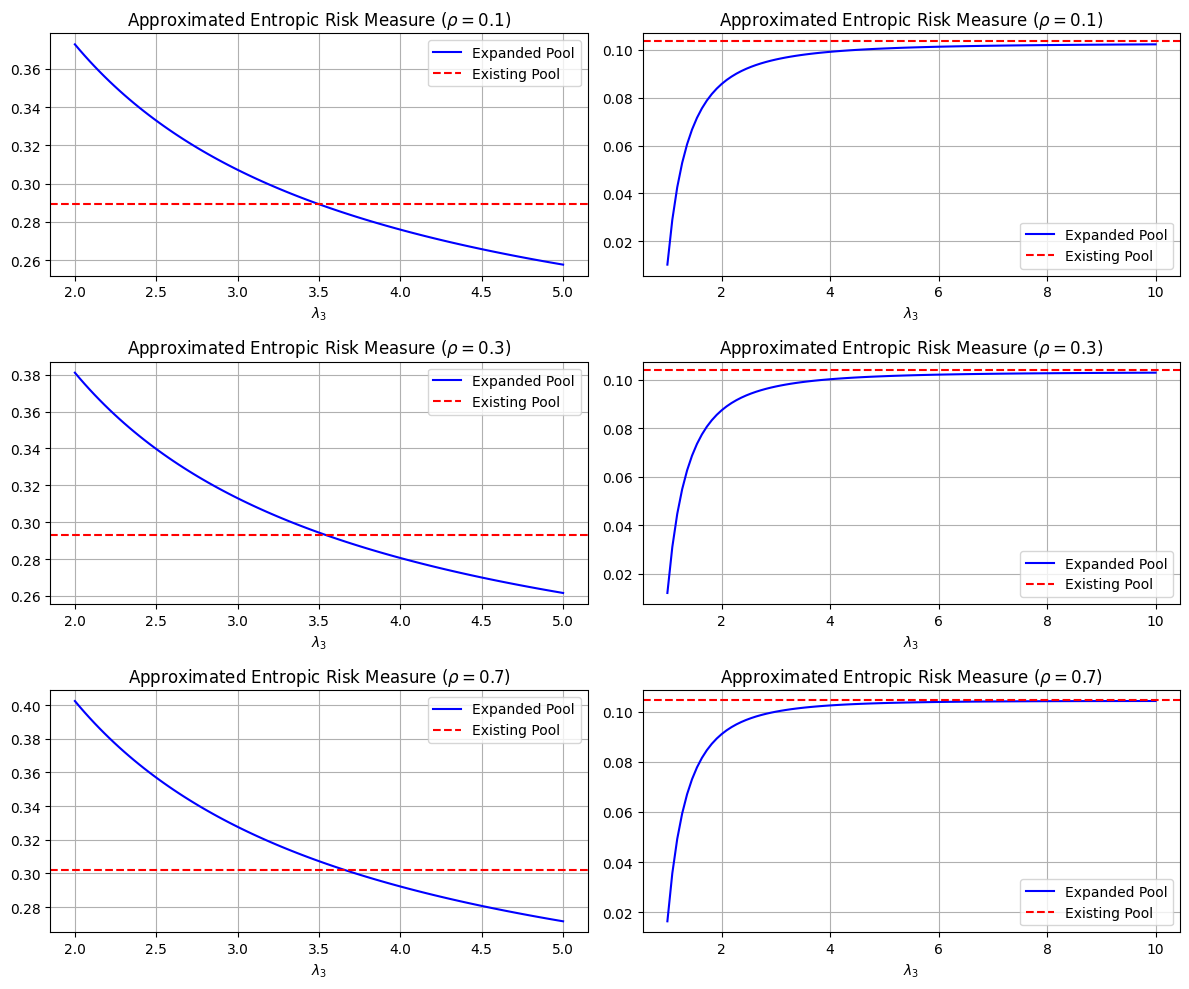
\includegraphics[width=\linewidth]{Figures/exp_together.png}
\label{app:fig:exp_together}
\end{figure}

\subsection{Results}\label{app:simul_result}
The presented simulations assume an existing risk pool comprising two members and consider the main case of common pair correlation ($\rho=0.1$, $0.3,$ and $0.7$) and common agents' risk tolerance (equal to one). Figure \ref{app:fig:exp_together} presents the simulation results for exponential distributions: The loss distributions of the existing members and the candidate follow exponential distributions with parameters $\lambda_1,$ $\lambda_2$, and $\lambda_3$ respectively. On the left panels in Figure \ref{app:fig:exp_together} the fairness principle is imposed, where $\lambda_1=3$ and $\lambda_2=5$. Therein, the risk measure of the expanded pool is shown to decrease with respect to $\lambda_3$ confirming that candidates with lower variance are more likely to be accepted under the fairness principle. In contrast, on the right panels in Figure \ref{app:fig:exp_together}, the risk measure of the expanded pool increases with respect to $\lambda_3$ under the equilibrium principle, where $\lambda_1=10$ and $\lambda_2=15$. The observation that candidates with sufficiently high variance are always accepted under this equilibrium pricing aligns with the analytic formulas under normally distributed risks. We also verify that higher correlation means higher risk measure under the expanded risk pool.

\begin{figure}[t]
\caption{Finite sample approximations of risk measures for the existing and expanded pools, based on Pareto distribution, under the fairness and equilibrium principles with varying values of $\alpha_3.$}
\centering
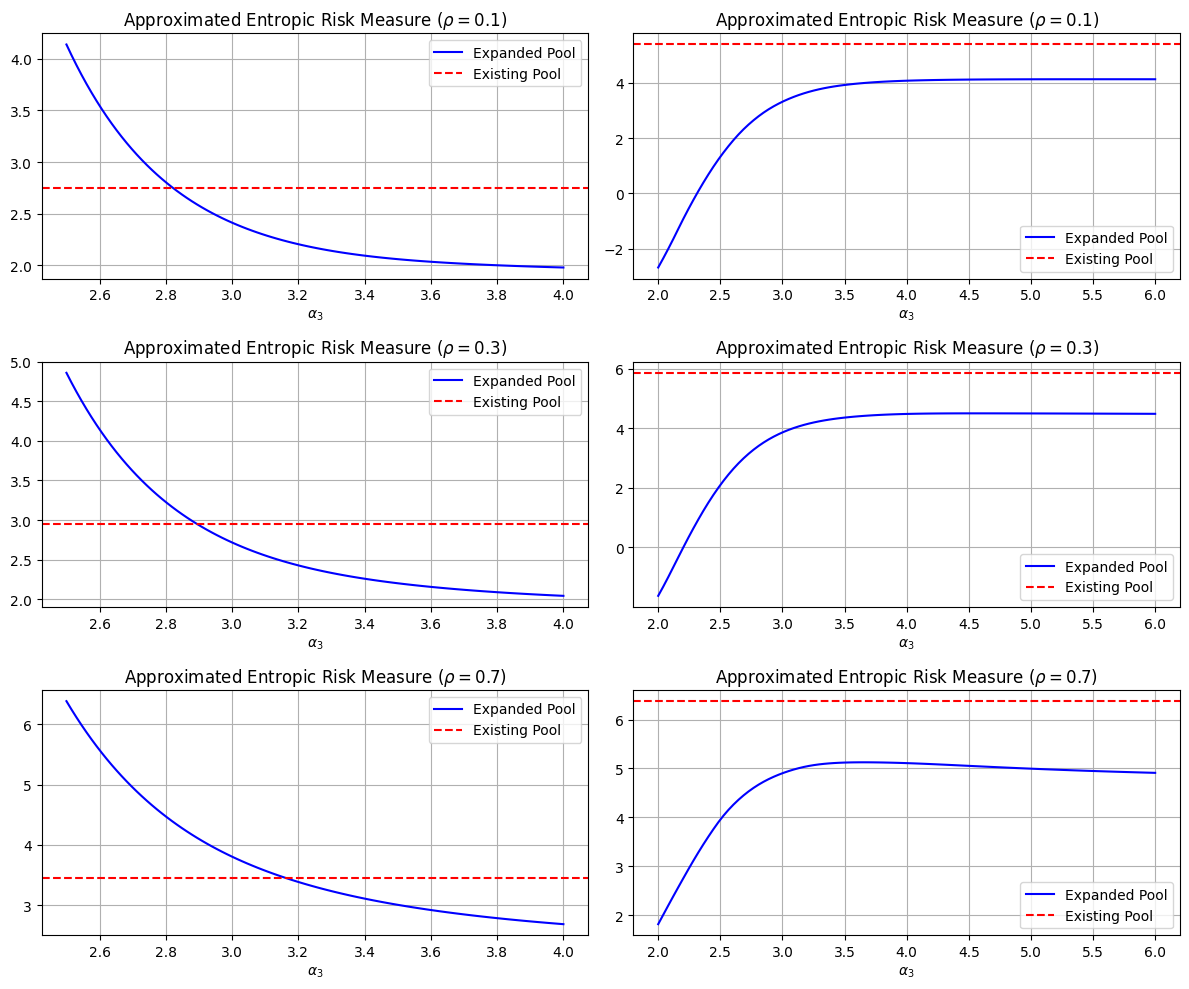
\includegraphics[width=\linewidth]{Figures/Pareto_together.png}
\label{app:fig:pareto_together}
\end{figure}

In Figure \ref{app:fig:pareto_together}, the Pareto distribution is used for the simulation. Recall that the linear risk-sharing rule is indeed optimal for any bounded approximated version of the Pareto distribution. Hence, for any practical perspective the numerical simulations of agents' risk measures could be used to (at least) examine the qualitative take-home message of our work.

With the scale parameter fixed at 1, the shape parameters are given by $\alpha_1=3,$ $\alpha_2=4$, and $\alpha_3$ for the existing members and the candidate, respectively. In Figure \ref{app:fig:pareto_together}, the results align with previous findings: candidates with lower risk are preferred under the fairness principle, whereas candidates with sufficiently high risk are consistently favored under the equilibrium principle. Notably, the upward slope followed by a downward slope (on the right panels in Figure \ref{app:fig:pareto_together}) illustrates the prediction from the main text, indicating the possibility of accepting candidates with either sufficiently low or sufficiently high risk under the equilibrium principle. The qualitative similarity of results obtained using the Pareto and normal distributions indicates that these findings are robust for heavy-tailed distributions as well.

\begin{figure}[t]
\caption{Finite sample approximations of risk measures for the existing and expanded pools, based on the Gamma distribution, under the fairness and equilibrium principles with varying values of $\theta_3.$}
\centering
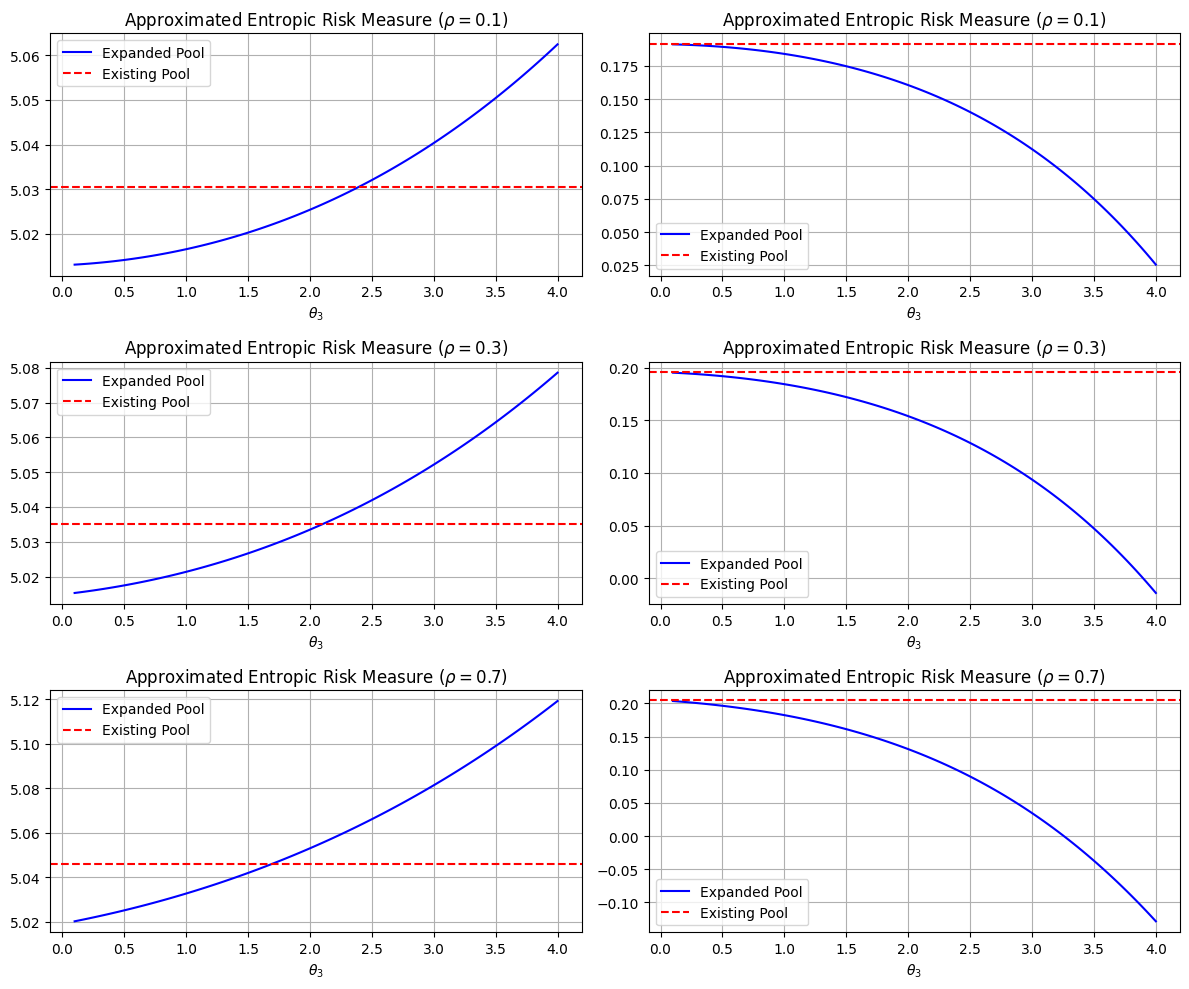
\includegraphics[width=\linewidth]{Figures/gamma_together.png}
\label{app:fig:gamma_together}
\end{figure}

Finally, Section \ref{app:fig:gamma_together} illustrates an example of our simulation under Gamma distribution. In this example, we assume a fixed shape parameter of 1, with scale parameters set as $\theta_1=1,$ $\theta_2=2,$ while $\theta_3$ varies. Consistent with earlier cases, the simulations in Figure \ref{app:fig:gamma_together} confirm that under the fairness principle (on the left panels), candidates with lower risk are preferred, while under the equilibrium principle (on the right panels), candidates with higher risk are favored.

The simulation results demonstrated that the qualitative conclusions remain consistent across normal and other distributions, even when applied to settings that differ from the normal distribution. For instance, in the exponential distribution, the single parameter $\lambda$ simultaneously affects both the mean and the variance, whereas in the normal distribution, variance is distribution's parameter. This consistency suggests that the conclusions are likely to extend to other distributions as well, despite the involved analytical complexities.

% \begin{figure}[t]
% \centering
% \caption{\textcolor{red}{combine, 3 by 2 matrix, just approximated risk measures}Risk measures for the existing pool and the expanded pool under fairness principle with varying values of $\lambda_3$. The parameters are given by $\lambda_1=3,$ $\lambda_2=5$, $\rho=(0.1,0.3,0.7),$ and $\delta=1$.}
% \includegraphics[width=1\linewidth]{Figures/exp_cor.png}
% \label{fig:exp_cor}
% \end{figure}
% Figure \ref{fig:exp_equi} is also consistent with the normal distribution case in the sense that as the candidate with sufficiently high variance is always going to be accepted.
% \begin{figure}[t]
% \centering
% \caption{Risk measures for the existing pool and the expanded pool under equilibrium principle with varying values of $\lambda_3$. The parameters are given by $\lambda_1=10,$ $\lambda_2=15$, $\rho=(0.1,0.3,0.7),$ and $\delta=1$.}
% \includegraphics[width=1\linewidth]{Figures/exp_equi.png}
% \label{fig:exp_equi}
% \end{figure}

% \subsection{Pareto Distribution}\label{app:simul_pareto}
% The simulation of Pareto distributions is also presented, under the same assumptions- fixed pairwise correlation $\rho$ and risk tolerance $\delta$. It is assumed that two existing agents and a candidate have loss distributions which follow Pareto distributions with the same scale parameter $x_m$ and the shape parameter $\alpha_1$, $\alpha_2$, and $\alpha_3$ respectively. Figure \ref{fig:pareto_cor} illustrates that as the $\alpha_3$ increases, the risk measure of expanded pool decreases. Since the variance of Pareto distribution decreases with $\alpha_3$ for $\alpha_3>2,$ the result aligns with our expectation that the candidate with lower variance is more likely to be accepted under the fairness principle.
% \begin{figure}[t]
% \centering
% \caption{Finite sample approximations of risk measures for the existing pool and the expanded pool under fairness principle with varying values of $\alpha_3$. The parameters are given by $\alpha_1=3,$ $\alpha_2=4$, $\rho=(0.1,0.3,0.7),$ and $\delta=1$.}
% \includegraphics[width=1\linewidth]{Figures/pareto_cor.png}
% \label{fig:pareto_cor}
% \end{figure}
% In Figure \ref{fig:pareto_equi}, the result is in line with that in a normal distribution case, as increasing risk measure of expanded pool with respect to $\alpha_3$ implies the candidate with higher variance is more likely to be accepted.
% \begin{figure}[htp!]
% \centering
% \caption{Finite sample approximations of risk measures for the existing pool and the expanded pool under equilibrium principle with varying values of $\alpha_3$. The parameters are given by $\alpha_1=3,$ $\alpha_2=4$, $\rho=(0.1,0.3,0.7),$ and $\delta=1$.}
% \includegraphics[width=\linewidth]{Figures/pareto_equi.png}
% \label{fig:pareto_equi}
% \end{figure}

% \subsection{Gamma Distribution}\label{app:simul_gamma}
% The simulation of Gamma distributions is presented under the fixed pairwise correlation $\rho$ and risk tolerance $\delta$. Two agents and a candidate have loss distributions modeled by Gamma distributions with the same shape parameter $\alpha$ and the scale parameters $\theta_1$, $\theta_2$, and $\theta_3$, respectively. Since the variance of Gamma distribution increases with $\theta_3,$ Figure \ref{fig:gamma_cor} confirms that the fairness principle prefers the candidate with lower variance.
% % \begin{figure}[t]
% % \centering
% % \caption{Risk measures for the existing pool and the expanded pool under fairness principle with varying values of $\theta_3$. The parameters are given by $\theta_1=1,$ $\theta_2=2$, $\rho=(0.1,0.3,0.7),$ and $\delta=1$.}
% % \includegraphics[width=1\linewidth]{Figures/gamma_cor.png}
% % \label{fig:gamma_cor}
% % \end{figure}
% It can be seen from Figure \ref{fig:gamma_equi} that the risk measure of expanded pool decreases with $\theta_3.$ This confirms that the candidate with higher variance is preferred under the equilibrium principle.
% % \begin{figure}[htp!]
% % \centering
% % \caption{Risk measures for the existing pool and the expanded pool under equilibrium principle with varying values of $\theta_3$. The parameters are given by $\theta_1=1,$ $\theta_2=2$, $\rho=(0.1,0.3,0.7),$ and $\delta=1$.}
% % \includegraphics[width=\linewidth]{Figures/gamma_equi.png}
% % \label{fig:gamma_equi}s
% % \end{figure}
\bigskip

\section{Supplementary Materials for Section \ref{sec:expansion}}\label{pf:main}
\subsection{Proofs of Section \ref{sec:expansion}}
\paragraph{Proof of Theorem \ref{thm:maintheorem}}
\ 

Theorem \ref{thm:optimalsharing} implies that risk-sharing of $n$ agents is proportional and determined by $\lambda_{n,i}$. Specifically, the risk allocated to the agent $i$ is
\[
\lambda_{n,i}S_n\sim\Normal\left(\lambda_{n,i}m_{n},\lambda_{n,i}^2s_{n}^2\right),
\]
where 
$s_{n+1}^2=s_n^2+\sigma_{n+1}^2+2\rho(S_n,X_{n+1})s_n\sigma_{n+1}.$ 
By the fairness principle, the cash transfers of agent $i$ in the pools with $n$ and $n+1$ agents are
\begin{align*}
&\pi_{n,i}=\lambda_{n,i}m_{n}-\mu_i;\\
&\pi_{n+1,i}=\lambda_{n+1,i}m_{n+1}-\mu_i,
\end{align*}
respectively. The entrance of the candidate benefits the existing agent $i$ if and only if 
\begin{align*}
\CE_i\left(\lambda_{n,i}S_n-\pi_{n,i}\right)\geq\CE_i\left(\lambda_{n+1,i}S_{n+1}-\pi_{n+1,i}\right).
\end{align*}
It follows that
\begin{equation}\label{eq:ratiodiff}
\frac{s_{n}^2}{\Delta_{n}^2}\geq\frac{s_{n+1}^2}{\Delta_{n+1}^2} 
\end{equation}
Similarly, the candidate is willing to participate in the pool if and only of
\begin{align*}
\CE_{n+1}\left(X_{n+1}\right)\geq\CE_{n+1}\left(\lambda_{n+1,n+1}S_{n+1}-\pi_{n+1,n+1}\right).
\end{align*}
It follows that
\begin{equation}\label{eq:strong_candidate}
\frac{\sigma_{n+1}^2}{\delta_{n+1}^2}\geq \frac{s_{n+1}^2}{\Delta_{n+1}^2}. \end{equation}


\paragraph{Proof of Corollary \ref{cor:correlation}}
\

Since $s_{n+1}^2=s_n^2+\sigma_{n+1}^2+2\rho(S_n,X_{n+1})s_n\sigma_{n+1},$ rewriting the inequality \eqref{eq:ratiodiff} with respect to $\rho(S_n,X_{n+1})$ gives
\begin{gather*}
\rho(S_n,X_{n+1})\leq\frac{(\Delta_{n+1}^2-\Delta_n^2)s_{n}^2-\Delta_n^2\sigma_{n+1}^2}{2\Delta_n^2s_{n}\sigma_{n+1}}.
\end{gather*}
In a similar manner, rewriting the inequality \eqref{eq:strong_candidate} with respect to $\rho(S_n,X_{n+1})$ gives
\[
\rho(S_n,X_{n+1})\leq\frac{(\Delta_{n+1}^2-\delta_{n+1}^2)\sigma_{n+1}^2-\delta_{n+1}^2s_{n}^2}{2\delta_{n+1}^2s_n\sigma_{n+1}}.
\]


\paragraph{Proof of Corollary \ref{cor:acceptance}}
\

Recall that $\Sigma_{n}:=\sum_{i=1}^n\sigma_{i}.$ By the normality assumption and the common pairwise correlation assumption,
\[
\rho(S_n,X_{n+1})=\sum_{i=1}^{n}\frac{\Cov(X_i,X_{n+1})}{s_{n}\sigma_{n+1}}=\frac{\rho\Sigma_{n}}{s_{n}}.
\]
Thus, \eqref{eq:ratiodiff} becomes
\[\sigma_{n+1}^2+2\rho\Sigma_{n}\sigma_{n+1}-(\Delta_{n+1}^2/\Delta_{n}^2-1)s_{n}^2\leq 0,
\]
which is equivalent to
\[
0<\sigma_{n+1}\leq  -\rho\Sigma_{n}+\sqrt{\left(\rho\Sigma_{n}\right)^2+\left(\frac{\Delta_{n+1}^2}{\Delta_{n}^2}-1\right)s_{n}^2}.
\]
Moreover, \eqref{eq:strong_candidate} becomes
\[
(\Delta_{n+1}^2-\delta_{n+1}^2)\sigma_{n+1}^2-2\rho\delta_{n+1}^2\sigma_{n+1}\Sigma_{n}-\delta_{n+1}^2s_{n}^2\geq0.
\]
which is equivalent to 
\[
\sigma_{n+1}\geq \delta_{n+1}^2\frac{\rho\Sigma_{n}+\sqrt{\left(\rho\Sigma_{n}\right)^2+(\Delta_{n+1}^2-\delta_{n+1}^2)s_{n}^2}}{\Delta_{n+1}^2-\delta_{n+1}^2}>0.
\]
Combining two inequalities gives the desired bounds for $\sigma_{n+1}.$
\bigskip

\paragraph{Proof of Remark \ref{rmk:either}}
\

It suffices to show that for any given $\boldsymbol{\delta}=(\delta_i)_{1\leq i\leq n}$ and $\boldsymbol{\sigma}=(\sigma_i)_{1\leq i\leq n},$ there is no $\sigma_{n+1}$ such that 
\[
\max\left\{ \frac{(\Delta_{n+1}^2-\Delta_n^2)s_{n}^2-\Delta_n^2\sigma_{n+1}^2}{2\Delta_n^2s_{n}\sigma_{n+1}},\frac{(\Delta_{n+1}^2-\delta_{n+1}^2)\sigma_{n+1}^2-\delta_{n+1}^2s_{n}^2}{2\delta_{n+1}^2s_n\sigma_{n+1}}\right\}
<1.
\]
Two functions intersect when
\[
\frac{(\Delta_{n+1}^2-\Delta_n^2)s_{n}^2-\Delta_n^2\sigma_{n+1}^2}{2\Delta_n^2s_{n}\sigma_{n+1}}=\frac{(\Delta_{n+1}^2-\delta_{n+1}^2)\sigma_{n+1}^2-\delta_{n+1}^2s_{n}^2}{2\delta_{n+1}^2s_n\sigma_{n+1}},
\]
which occurs at 
\[
\sigma_{n+1}^*=\frac{\delta_{n+1}s_n}{\Delta_n}.
\] 
Note that
\[
\left.\frac{(\Delta_{n+1}^2-\Delta_n^2)s_{n}^2-\Delta_n^2\sigma_{n+1}^2}{2\Delta_n^2s_{n}\sigma_{n+1}}\right|_{\sigma_{n+1}=\sigma_{n+1}^*}=1.
\]
But if $\sigma_{n+1}<\delta_{n+1}s_n/\Delta_n$, then 
\[
\frac{(\Delta_{n+1}^2-\Delta_n^2)s_{n}^2-\Delta_n^2\sigma_{n+1}^2}{2\Delta_n^2s_{n}\sigma_{n+1}}>1,
\]
% because
% \[
% \frac{\partial}{\partial \sigma_{n+1}}\left(\frac{(\Delta_{n+1}^2-\Delta_n^2)s_{n}^2-\Delta_n^2\sigma_{n+1}^2}{2\Delta_n^2s_{n}\sigma_{n+1}}\right)=-\frac{(\Delta_{n+1}^2-\Delta_n^2)s_{n}}{2\Delta_n^2\sigma_{n+1}^2}-\frac{1}{2s_{n}}<0.
% \]
and if $\sigma_{n+1}>\delta_{n+1}s_n/\Delta_n$, we have 
\[
\frac{(\Delta_{n+1}^2-\delta_{n+1}^2)\sigma_{n+1}^2-\delta_{n+1}^2s_{n}^2}{2\delta_{n+1}^2s_n\sigma_{n+1}}>1.
\]
% Thus, for any $\sigma_{n+1},$ we have
% \[
%     \max\left\{ \frac{(\Delta_{n+1}^2-\Delta_n^2)s_{n}^2-\Delta_n^2\sigma_{n+1}^2}{2\Delta_n^2s_{n}\sigma_{n+1}},\frac{(\Delta_{n+1}^2-\delta_{n+1}^2)\sigma_{n+1}^2-\delta_{n+1}^2s_{n}^2}{2\delta_{n+1}^2s_n\sigma_{n+1}}\right\}
%    \geq 1,
% \]
This implies the desired result.
\bigskip 
\paragraph{Proof of Theorem \ref{thm:weakconsensus}}
\\ \


The aggregate risk after the expansion is 
\[
S_{n+1}=\sum_{j=1}^{n+1}X_j\sim\Normal(m_{n+1},s_{n+1}^2),
\]
where
\[
m_{n+1}=\sum_{j=1}^{n+1}\mu_j\quad\text{ and }\quad s_{n+1}^2=s_n^2+\sigma_{n+1}^2+2\rho(S_n,X_{n+1})s_n\sigma_{n+1}.
\]
By Theorem \ref{thm:optimalsharing}, the risk allocated to the agent $i$ is
\begin{align*}
\lambda_{n+1,i}S_{n+1}\sim\Normal\left(\lambda_{n+1,i}m_{n+1},\lambda_{n+1,i}^2s_{n+1}^2\right).
\end{align*}
By the fairness principle,
\[
\pi_{n+1,i}=\lambda_{n+1,i}m_{n+1}-\mu_i.
\]
The existing agent $i$ will leave the risk pool if 
\begin{align*}
\CE_{i}[X_{i}]\leq\CE_{i}[\lambda_{n+1,i}S_{n+1}-\pi_{n+1,i}],
\end{align*}
which is equivalent to
\begin{gather}
\frac{\sigma_{i}^2}{\delta_i^2}
\leq \frac{s_{n+1}^2}{\Delta_{n+1}^2}.\label{ineq:weak}
\end{gather}
Rewriting \eqref{ineq:weak} with respect to $\rho(S_n,X_{n+1})$ gives
\[
\rho(S_n,X_{n+1})\geq\frac{\Delta_{n+1}^2\sigma_i^2-\delta_i^2\sigma_{n+1}^2-\delta_i^2s_{n}^2}{2\delta_i^2s_n\sigma_{n+1}}.
\]


% \subsection{Proof: Corollary \ref{cor:asymtotic}}
%     Note
% \[
% \frac{\Delta_{n+1}^2\sigma_i^2-\delta_i^2\sigma_{n+1}^2-\delta_i^2s_{n}^2}{2\delta_i^2s_n\sigma_{n+1}}=\frac{\Delta_{n+1}^2\left(\frac{\sigma_{i}}{\delta_i}\right)^2-s_n^2-\sigma_{n+1}^2}{2s_n\sigma_{n+1}}.
% \]

% Then, we investigate the limit of the condition in Theorem \ref{cor:acceptance}. 
% \[
% \lim_{n\to\infty}\frac{\Delta_{n+1}^2\left(\frac{\sigma_{i}}{\delta_i}\right)^2-s_n^2-\sigma_{n+1}^2}{2s_n\sigma_{n+1}}.
% \]
% Thus,
% \[
% \lim_{n\to\infty}\frac{\Delta_{n+1}^2\left(\frac{\sigma_{i}}{\delta_i}\right)^2-s_n^2-\sigma_{n+1}^2}{2s_n\sigma_{n+1}}=-\infty.
% \]

% \subsection{Proof: Corollary \ref{cor:samecor}}

% Since $\rho(X_i,X_j)=\rho$ for all $i,j=1,2,...,n+1$,
% \begin{align*}
% \rho_{n, n+1}&=\frac{\Cov(S_{n},X_{n+1})}{s_n\sigma_{n+1}}\\
% &=\frac{\rho\sigma_{n+1}\Sigma_n}{s_n\sigma_{n+1}}.
% \end{align*}
% % Moreover, note that
% % \[
% % s_n^2=\sum_{i=1}^n \sigma_i^2+\sum_{i\neq j}^n 2\Cov(X_i,X_j)=\sum_{i=1}^n \sigma_i^2+2{n\choose 2}C.
% % \]
% From Theorem \ref{thm:weakconsensus}, it follows that
% \begin{gather*}
%     \frac{\rho\sigma_{n+1}\Sigma_n}{s_n\sigma_{n+1}}\geq\frac{\Delta_{n+1}^2\left(\frac{\sigma_{i}}{\delta_i}\right)^2-s_n^2-\sigma_{n+1}^2}{2s_n\sigma_{n+1}}\\
%     \left(\frac{\sigma_i}{\delta_i}\right)^2\leq\frac{2\rho\sigma_{n+1}\Sigma_n+\sigma_{n+1}^2+s_n^2}{\Delta_{n+1}^2}.
% \end{gather*}

% \subsection{Proof for Corollary \ref{cor:acceptregion2}}
% Let the condition for the current members be
% \[
%     f_1:=\frac{s_{n+1}^2}{\Delta_{n+1}^2}-\frac{s_{n}^2}{\Delta_{n}^2}\left(\leq 0, \,\text{ for acceptance}\right).
% \]
% Then,
% \[
%     \frac{df_1}{d\rho}=2\Sigma_{n}\sigma_{n+1}-(\Delta_{n+1}^2/\Delta_{n}^2-1)\sum_{j}\sum_{i\neq j}\sigma_i\sigma_j\geq0.
% \]
% On the other hand, for the candidate, the condition becomes
% \[
% f_2:=\frac{s_{n+1}^2}{\Delta_{n+1}^2}-\frac{\sigma_{n+1}^2}{\delta_{n+1}^2}\left(\leq 0, \,\text{ to join}\right) 
% \]
% It follows that $df_2/d\rho\geq0$ if and only if
% \[
%     \frac{df_2}{d\rho}=2\delta_{n+1}^2\sigma_{n+1}\Sigma_{n}+\sum_{j}\sum_{i\neq j}\sigma_i\sigma_j\geq0.
% \]

% %\subsection{Proof: Theorem \ref{thm:twoapp}}
% %There could be three cases.
% %\begin{enumerate}
%  %   \item Suppose that no one is accepted, i.e., $U(N)<U(N\cup \{i\})$ and $U(N)<U(N\cup \{j\})$. Thus, the order does not matter.
%   %  \item Suppose that only one agent is accepted. Without loss of generality, we can assume that the agent $i$ is accepted, and then the agent $j$ is not accepted. For the reversed order, if the agent $j$ is not accepted, it follows that the agent $i$ will be accepted and the agent $j$ will not be accepted as with the assumption. If the agent $j$ is accepted, then we have to prove that the agent $i$ will not be accepted. It is proved by Theorem \ref{lem:sameindex}, $U(N\cup \{i\})<U(N\cup \{i,j\})$ if and only if $U(N\cup \{j\})<U(N\cup \{i,j\})$, which implies that the agent $i$ will not be accepted. Thus, the order does not matter.
%    % \item Suppose that both agents are accepted. Without loss of generality, assume that the agent $i$ is accepted, and then the agent $j$ is accepted. If the agent $j$ is not accepted, the agents $i$ and $j$ will be accepted as the same order. If the agent $j$ is accepted, by Theorem \ref{lem:sameindex}, the agent $i$ will be accepted. Thus, the order does not matter. 

%     %  The proof by contradiction is used. Let E=\{1,2,...,n\}. Suppose that the agent $i$ is accepted and $j$ is also accepted. Then,
%     %\[
% % \min_{i=E\cup \{i,j\}}\left(\frac{\sigma_i}% % {\delta_i}\right)^2\geq \frac{s_{n+2}^2}%{\Delta_{n+2}^2},
% %\]
% %If $j$ is accepted and $i$ is not accepted,
% %\[
% %\min_{i=E\cup \{i,j\}}\left(\frac{\sigma_i}%{\delta_i}\right)^2< \frac{s_{n+2}^2}{\Delta_{n+2}^2},
% %\]
% % Since 
% % \[
% % \min_{i=N_i\cup \{j\}} \left(\frac{\sigma_i}{\delta_i}\right)^2=\min_{i=N_j\cup \{i\}} \left(\frac{\sigma_i}{\delta_i}\right)^2,
% % \]
% %It follows that
% %\[
% %\frac{s_{n+2}^2}{\Delta_{n+2}^2}>\frac{s_{n+2}^2}%{\Delta_{n+2}^2},\]
% %which is a contradiction.
% % Comparing the inequality,
% % \begin{align*}
% %     \left(2\rho\sigma_{j}\Sigma_{N_i}+\sigma_{j}^2+s_{N_i}^2\right) - \left(2\rho\sigma_{i}\Sigma_{N_j}+\sigma_{i}^2+s_{N_j}^2\right)>0\\
% %     \left(2\rho\sigma_{j}\sum_{k\in N_i}\sigma_k+\sigma_{j}^2+\left(\sum_{k\in N_i}\sigma_k^2+2\rho\sum_{\substack{k<l \\ k,l\in N_i}}\sigma_k\sigma_l\right)\right)- \left(2\rho\sigma_{i}\sum_{k\in N_j}\sigma_k+\sigma_{i}^2+\left(\sum_{k\in N_j}\sigma_k^2+2\rho\sum_{\substack{k<l \\ k,l\in N_j}}\sigma_k\sigma_l\right)\right)> 0\\
% %     \left(\sigma_{j}^2+\sum_{k\in N_i}\sigma_k^2-\sigma_{i}^2-\sum_{k\in N_j}\sigma_k^2\right)+\left(2\rho\sigma_{j}\sum_{k\in N_i}\sigma_k+2\rho\sum_{\substack{k<l \\ k,l\in N_i}}\sigma_k\sigma_l-2\rho\sigma_{i}\sum_{k\in N_j}\sigma_k-2\rho\sum_{\substack{k<l \\ k,l\in N_j}}\sigma_k\sigma_l\right)=0<0,
% % \end{align*}
% % which is a contradiction.
% %\end{enumerate}
\bigskip

\section{Supplementary Materials for Section \ref{sec:reinsurance}}\label{App:B}

\subsection{Maximum Extra Premium}\label{app:extra_prem}
Thanks to the combined effect of risk diversification and reinsurance, each member is in fact willing to pay an extra premium, on top of the actuarially fair premium. This will make the total reinsurance premium equal to $pr^{(n)}+c^{(n)}=\sum_{i=1}^n\, (pr_{n,i} +c_i)=pr^{(n)}+\mathbb{E}[ (S_n-K)_+],$ where $pr_{n,i}$ is the extra premium allocated to agent $i$, such that $\sum_{i=1}^n pr_{n,i}=pr$. From a different perspective, the above arguments could yield the maximum reinsurance premium $pr^*_n$ that the group is willing to pay and still achieve a positive aggregate risk reduction. For this, we simply consider $pr^*_n$ as the total reduction that the actuarially fair-priced reinsurance gives to the group. This is the subject of the following statement. 

{\it Under the normality assumption and actuarial fairness, the maximum extra premium that the pool is willing to pay is given as
\begin{equation}\label{eq:maximum premium}
pr^*_n= \Delta_n\left(\frac{1}{2}\left(\frac{s_{n}}{\Delta_{n}}\right)^2- l\left(\frac{s_{n}}{\Delta_{n}};\beta\right)\right)>0,
\end{equation}
where function $l(x;\beta)$ is given as
\[
l(x;\beta):=\log\left(e^{\frac{x^2}{2}}\Phi\left(\beta-x\right)+e^{\beta x}(1-\Phi(\beta))\right)+ x\left(\phi(\beta)-\beta(1-\Phi(\beta))\right).
\]
}
The proof is as follows. Let the extra premium (on top of fair price) paid to the reinsurer by the pool be equal to $pr^{(n)}$. We first calculate the aggregate risk measure without reinsurance:
\begin{align*}
\sum_{i=1}^n \rho_i[\textrm{Without Reinsurance}]&=\sum_{i=1}^n\rho_i\left[\lambda_{n,i}S_n+\pi_{n,i}\right]=\sum_{i=1}^n\left(\lambda_{n,i}m_{n}+\frac{\lambda_{n,i}}{2\Delta_{n}}s_{n}^2+\mu_i-\lambda_{n,i}m_{n}\right)\\
&=m_n+\frac{s_{n}^2}{2\Delta_{n}}.
\end{align*}
With the reinsurance, the aggregate risk measure is
\begin{align*}
\sum_{i=1}^n\rho_i[\textrm{With Reinsurance}]=\sum_{i=1}^n\rho_i\left[\lambda_{n,i}\overline{S}_{n}+pr_{n,i}-c_i\right]=\sum_{i=1}^n\rho_i\left[\lambda_{n,i}\overline{S}_{n}\right]+\pi_{n,i}+pr^{(n)}+c^{(n)}.
\end{align*}
The first part of the above equation is written as 
\begin{align*}
\sum_{i=1}^n\CE_i\left[\lambda_{n,i}\overline{S}_{n}\right]
&=\sum_{i=1}^n\delta_i\log\left(\left(e^{\frac{1}{\Delta_{n}}m_n+\frac{1}{2\Delta_{n}^2}s_{n}^2}\right)\Phi\left(\beta-\frac{1}{\Delta_{n}}s_{n}\right)+e^{\frac{1}{\Delta_{n}}K}(1-\Phi(\beta))\right)\\
&=m_n+\sum_{i=1}^n\delta_i l_{n}=m_n+\Delta_nl_n,
\end{align*}
where \[l_n:=l\left(\frac{s_{n}}{\Delta_{n}};\beta\right)=\log\left(e^{\frac{s_{n}^2}{2\Delta_{n}^2}}\Phi\left(\beta-\frac{s_{n}}{\Delta_{n}}\right)+e^{\beta\frac{s_{n}}{\Delta_{n}}}(1-\Phi(\beta))\right).\]
Since for the internal cash transfer it holds that $\sum_{i=1}^n\pi_{n,i}=0$, the total pool's cash payment to the reinsurance is 
\begin{align*}
pr^{(n)}+c^{(n)}&=pr^{(n)}+\EE[ (S_n-K)_+]=pr^{(n)}+(\EE[S_n|S_n\geq K]-K)\prob{S_n\geq K}\\
&=pr^{(n)}+\left(m_n+\frac{s_n\phi(\beta)}{1-\Phi(\beta)}-K\right)(1-\Phi(\beta))\\
&=pr^{(n)}+m_n(1-\Phi(\beta))+s_n\phi(\beta)-(m_n+\beta s_n)(1-\Phi(\beta))\\
&=pr^{(n)}+s_n(\phi(\beta)-\beta (1-\Phi(\beta))).
\end{align*}
Therefore,
\[
\sum_{i=1}^n\CE_i[\textrm{With Reinsurance}]=m_n+\Delta_nl_{n}+pr^{(n)}+s_n(\phi(\beta)-\beta (1-\Phi(\beta))).
\]
The maximum acceptable extra premium $pr^*$ is the one that makes aggregate risk measures equal:
\[\sum_{i=1}^n \rho_i[\textrm{Without Reinsurance}]=\sum_{i=1}^n \rho_i[\textrm{With Reinsurance}],\]
which gives \eqref{eq:maximum premium}.


\subsection{Proofs of Section \ref{sec:reinsurance}}

\paragraph{Proof of Theorem \ref{thm:fair_reinsualwaysbetter}}
\

Define 
\[
g(x;\beta)=\frac{x^2}{2}-l(x;\beta).
\]
It suffices to show that $g(x;\beta)\geq0$ for all $x,\beta>0.$ Note that $g(0;\beta)=0$ for all $\beta.$ Fix $\beta>0.$ Then, 
\[
\frac{d}{dx}g(x;\beta)=x-\frac{xe^{x^2/2}\Phi(\beta-x)-e^{x^2/2}\phi(\beta-x)+\beta e^{x\beta}\Phi(-\beta)}{e^{x^2/2}\Phi(\beta-x)+e^{x\beta}\Phi(-\beta)}-\phi(\beta)+\beta\Phi(-\beta).
\]
Thus, $dg(x;\beta)/dx\geq 0$ if and only if
\begin{align}
\begin{split}
&xe^{x\beta}\Phi(-\beta)+e^{x^2/2}\phi(\beta-x)-\beta e^{x\beta}\Phi(-\beta)-\phi(\beta)e^{x^2/2}\Phi(\beta-x)\\
&-\phi(\beta)e^{x\beta}\Phi(-\beta)+\beta\Phi(-\beta)e^{x^2/2}\Phi(\beta-x)+\beta\Phi(-\beta)e^{x\beta}\Phi(-\beta)\geq 0.
\end{split}\label{ineq:gxmonotone}
\end{align}
Replacing $\phi(z)$ with $e^{-z^2/2}/\sqrt{2\pi}$ and multiplying $e^{-x\beta+\beta^2/2}$ to \eqref{ineq:gxmonotone} makes it equivalent to 
% \begin{align*}
%         &xe^{x\beta}\Phi(-\beta)+e^{x^2/2}e^{-(\beta-x)^2/2}/\sqrt{2\pi}-\beta e^{x\beta}\Phi(-\beta)-e^{-\beta^2/2}/\sqrt{2\pi}e^{x^2/2}\Phi(\beta-x)\\
%     &-e^{-\beta^2/2}/\sqrt{2\pi}e^{x\beta}\Phi(-\beta)+\beta\Phi(-\beta)e^{x^2/2}\Phi(\beta-x)+\beta\Phi(-\beta)e^{x\beta}\Phi(-\beta)\geq 0
% \end{align*}
% \begin{align*}
%         &xe^{\beta^2/2}\Phi(-\beta)+1/\sqrt{2\pi}-\beta e^{\beta^2/2}\Phi(-\beta)-e^{-x\beta}/\sqrt{2\pi}e^{x^2/2}\Phi(\beta-x)\\
%     &-1/\sqrt{2\pi}\Phi(-\beta)+\beta\Phi(-\beta)e^{x^2/2-x\beta+\beta^2/2}\Phi(\beta-x)+\beta\Phi(-\beta)e^{\beta^2/2}\Phi(-\beta)\geq 0
% \end{align*}
% Thus,
\begin{align}
\begin{split}
&xe^{\beta^2/2}\Phi(-\beta)+1/\sqrt{2\pi}+\beta e^{(x-\beta)^2/2}\Phi(-\beta)\Phi(\beta-x)+\beta\Phi^2(-\beta)e^{\beta^2/2}\\
&\geq\beta e^{\beta^2/2}\Phi(-\beta)+e^{x^2/2-x\beta}\Phi(\beta-x)/\sqrt{2\pi}+\Phi(-\beta)/\sqrt{2\pi}.\label{ineq:g(xbeta)proof}
\end{split}
\end{align}
Assume for now that $x>\beta$. In the view of \eqref{ineq:g(xbeta)proof}, we directly get that
\begin{gather*}
xe^{\beta^2/2}\Phi(-\beta)> \beta e^{\beta^2/2}\Phi(-\beta)\\
0.5/\sqrt{2\pi}>\Phi(-\beta)/\sqrt{2\pi}.
\end{gather*}
On the other hand, we it also holds that 
\[    0.5/\sqrt{2\pi}+\beta e^{(x-\beta)^2/2}\Phi(-\beta)\Phi(\beta-x)> e^{x^2/2-x\beta}\Phi(\beta-x)/\sqrt{2\pi}.\]
Indeed, the above inequality can be re-written as
\[
\frac{0.5}{\Phi(\beta-x)e^{x^2/2-x\beta}}+\sqrt{2\pi}\beta e^{\beta^2/2}\Phi(-\beta)> 1.
\]
Note that
\[
\frac{d}{dx}\Phi(\beta-x)e^{x^2/2-x\beta}=e^{x^2/2-x\beta}\phi(\beta-x)\left(\frac{(x-\beta)\Phi(\beta-x)}{\phi(\beta-x)}-1\right)
\]
By the Mill's ratio,
\[
\frac{(x-\beta)\Phi(\beta-x)}{\phi(\beta-x)}=\frac{(x-\beta)(1-\Phi(x-\beta))}{\phi(x-\beta)}<1.
\]
Since $d\Phi(\beta-x)e^{x^2/2-x\beta}/dx<0$ for all $x>\beta,$ 
\[
\frac{0.5}{\Phi(\beta-x)e^{x^2/2-x\beta}}+\sqrt{2\pi}\beta e^{\beta^2/2}\Phi(-\beta)> e^{\beta^2/2}+\sqrt{2\pi}\beta e^{\beta^2/2}\Phi(-\beta)> 1.
\]
Hence, we get the desired inequality when $x>\beta$.

Assume now that $0<x<\beta$. Rewriting \eqref{ineq:g(xbeta)proof},
\begin{align}
(x-\beta\Phi(\beta))e^{\beta^2/2}\Phi(-\beta)+\frac{\Phi(\beta)}{\sqrt{2\pi}}+\frac{\Phi(\beta-x)e^{x^2/2-x\beta}}{\sqrt{2\pi}}(\beta\sqrt{2\pi} e^{\beta^2/2}\Phi(-\beta)-1)\geq 0.\label{ineq:g(xbeta)proof2}
\end{align}
Note
\begin{align*}
&\frac{d}{dx}(x-\beta\Phi(\beta))e^{\beta^2/2}\Phi(-\beta)=e^{\beta^2/2}\Phi(-\beta)>0
\end{align*}
By the Mill's ratio,
\[
\beta\sqrt{2\pi} e^{\beta^2/2}\Phi(-\beta)=\beta\frac{1-\Phi(\beta)}{\frac{1}{\sqrt{2\pi}} e^{-\beta^2/2}}=\beta\frac{1-\Phi(\beta)}{\phi(\beta)}<1.
\]
Thus,
\begin{align*}
&\frac{d}{dx}\Phi(\beta-x)e^{x^2/2-x\beta}(\beta\sqrt{2\pi} e^{\beta^2/2}\Phi(-\beta)-1)\\
&=e^{x^2/2-x\beta}(\beta\sqrt{2\pi} e^{\beta^2/2}\Phi(-\beta)-1)(-\phi(\beta-x)+\phi(\beta-x)(x-\beta))>0.
\end{align*}
It follows that LHS of \eqref{ineq:g(xbeta)proof2} is non-decreasing with respect to $x.$ Then,
\begin{align*}
&(x-\beta\Phi(\beta))e^{\beta^2/2}\Phi(-\beta)+\frac{\Phi(\beta)}{\sqrt{2\pi}}+\frac{\Phi(\beta-x)e^{x^2/2-x\beta}}{\sqrt{2\pi}}(\beta\sqrt{2\pi} e^{\beta^2/2}\Phi(-\beta)-1)\\
&\geq \lim_{x\to0}(x-\beta\Phi(\beta))e^{\beta^2/2}\Phi(-\beta)+\frac{\Phi(\beta)}{\sqrt{2\pi}}+\frac{\Phi(\beta-x)e^{x^2/2-x\beta}}{\sqrt{2\pi}}(\beta\sqrt{2\pi} e^{\beta^2/2}\Phi(-\beta)-1)\\
&=\Phi(\beta)\Phi(-\beta)e^{\beta^2/2}\left(-\beta +\beta \right)\\
&=0.
\end{align*}
Since $dg(x;\beta)/dx$ is continuous and non-negative for $0<x<\beta$ and $x>\beta,$ it is also non-negative when $x=\beta.$ It follows that $dg(x;\beta)/dx\geq 0$ for all $x,\beta>0$. For all $x,\beta>0$ and hence 
\[
g(x;\beta)\geq g(0;\beta)=0.
\]

%Note that $g_{n,i}(0;\beta)=0$ for all $\beta$. Moreover, from Figure \ref{fig:Fx}, $dg_{n,i}(x;\beta)/dx\geq 0$ for all $\beta.$ Thus, $g_{n,i}(x;\beta)\geq 0$ for all $x$ and $\beta$. The whole plot is given in Figure \ref{fig:F}.

% \begin{figure}[htp!]
%     \begin{subfigure}[b]{0.40\textwidth}
%             \centering
%             \includegraphics[width=\textwidth]{Figures/DFdx.jpg}
%             \subcaption{}
%             \label{fig:Fx}
%     \end{subfigure}
%     \hfill
%     \begin{subfigure}[b]{0.40\textwidth}
%             \centering
%             \includegraphics[width=\textwidth]{Figures/FF.jpg}
%             \subcaption{}
%             \label{fig:F}
%     \end{subfigure}
%     \caption{\macom{In the figures you write $F$ instead of $g$. Also, I think that the 3D graph is sufficient to get our result. We do not need the first figure.}\skcom{I will fix this after I finish the proof. Maybe we do not need this if we are able to prove analytically?} Illustration of $\partial g(x,\beta)/\partial x$ and $g(x,\beta)$}
%     \label{fig:Fxbeta}
% \end{figure}
% % }


\paragraph{Proof of Theorem \ref{thm:rein_strong}}
\

For the existing members, it must hold that
\[
\CE_i[\textrm{n agents with reinsurance}]-\CE_i[\textrm{n+1 agents with Reinsurance}]\geq0,
\]
i.e.,
\begin{gather*}
f_{e,i}=\CE_i\left[\lambda_{n,i}\overline{S}_{n}-\pi_{n,i}-p_{n,i}\right]-\CE_i\left[\lambda_{n+1,i}\overline{S}_{n+1}-\pi_{n+1,i}-p_{n+1,i}\right]\geq0.
\end{gather*}
That is,
\begin{align*}
f_{e,i}=\delta_i l_{n}-\lambda_{n,i}s_n\left(\phi(\beta)-\beta(1-\Phi(\beta))\right)+\mu_i-\delta_i l_{n+1}+\lambda_{n+1,i}s_{n+1}\left(\phi(\beta)-\beta(1-\Phi(\beta))\right)-\mu_i\geq 0.
\end{align*}
Thus,
\[
f_{e,i}=\delta_{i}(l_{n}-l_{n+1})-(\lambda_{n,i}s_n-\lambda_{n+1,i}s_{n+1})(\phi(\beta)-\beta(1-\Phi(\beta))\geq0.
\]
Dividing by $\delta_{i}$ gives the desired result. On the other hand, for the candidate to join, it must hold that
\begin{gather*}
f_{c}=\CE_{n+1}\left[X_{n+1}\right]-\CE_{n+1}\left[\lambda_{n+1,n+1}\overline{S}_{n+1}-\pi_{n+1,n+1}-p_{n+1,n+1}\right]\geq0.
\end{gather*}
As above,
\[
f_{c}=\frac{1}{2\delta_{n+1}}\sigma_{n+1}^2-\delta_{n+1} l_{n+1}+\lambda_{n+1,n+1}s_{n+1}\left(\phi(\beta)-\beta(1-\Phi(\beta))\right).
\]

\paragraph{Proof of Theorem \ref{thm:acceptchange_candidate}}
\

To prove Theorem \ref{thm:acceptchange_candidate}, we need to prove the following statement.
\begin{figure}[t]
\centering
\caption{Contour plot of $l(x;\beta)$}
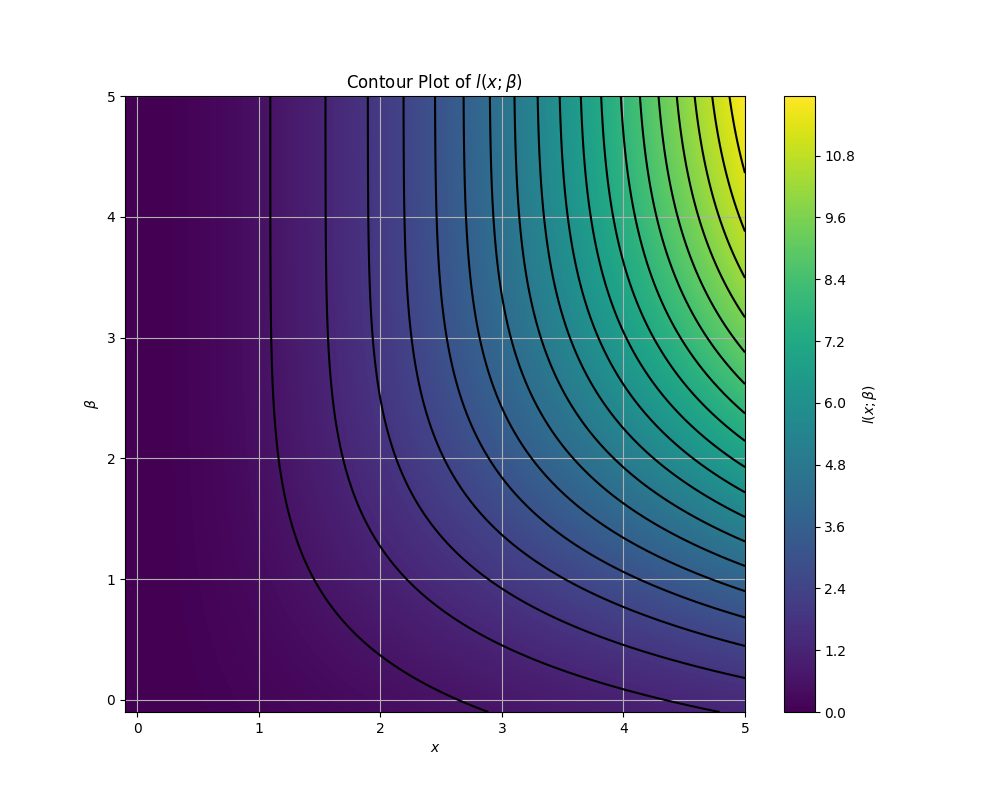
\includegraphics[width=0.65\textwidth]{Figures/contourlxb.png}
\label{fig:contourlxb}
\end{figure}

{\it Let $M:\mathbb{R}\mapsto\mathbb{R}$ be defined by $M(\beta):=\beta+\frac{1}{\beta}.$ The function $l(x;\beta)$ monotonically increases with respect to $x>0$, for all $\beta>0$, when $x\geq M(\beta).$}

It suffices to show that $l(x;\beta)\geq l(y;\beta)$ for any $x\geq y>M(\beta)$ and $\beta>0.$ 
\begin{align}
l(x;\beta)-l(y;\beta)=\log\left(\frac{e^{\frac{x^2}{2}}\Phi(\beta-x)+e^{\beta x}(1-\Phi(\beta))}{e^{\frac{y^2}{2}}\Phi(\beta-y)+e^{\beta y}(1-\Phi(\beta))}\right)+(x-y)(\phi(\beta)-\beta(1-\Phi(\beta))).\label{eq:lx minus ly}
\end{align}
Note that 
\[
\lim_{\beta\to\infty}\phi(\beta)-\beta(1-\Phi(\beta))=0\qquad\text{and}\qquad \frac{d}{d\beta}\left(\phi(\beta)-\beta(1-\Phi(\beta))\right)=\Phi(\beta)-1\leq 0.
\]
Thus, $\phi(\beta)-\beta(1-\Phi(\beta))\geq 0$ for all $\beta$ meaning that the second term in \eqref{eq:lx minus ly} is non-negative. Moreover, we readily get that 
\[
(e^{\beta x}-e^{\beta y})(1-\Phi(\beta))\geq 0,
\]
which means that it is only left to show that $e^{\frac{x^2}{2}}\Phi(\beta-x)$ is monotone for $x\geq M(\beta)$ and $\beta>0$. For this, we calculate
\[
\frac{d }{dx}\left(e^{\frac{x^2}{2}}\Phi(\beta-x)\right)=e^{\frac{x^2}{2}}(x\Phi(\beta-x)-\phi(\beta-x)),
\]
which is non-negative if 
\[
\frac{\Phi(\beta-x)}{\phi(\beta-x)}\geq \frac{1}{x}.
\]
The lower bound of the Mill's ratio implies that
% \[
% \frac{\Phi(\beta-x)}{\phi(\beta-x)}=\frac{1-\Phi(x-\beta)}{\phi(x-\beta)}\geq\frac{x-\beta}{(x-\beta)^2+1}.
% \]
\[
\frac{\Phi(\beta-x)}{\phi(\beta-x)}-\frac{1}{x}\geq\frac{x-\beta}{(x-\beta)^2+1}-\frac{1}{x}=\frac{\beta x-\beta^2 -1}{x((x-\beta)^2+1)}\geq 0
\]
% Then, 
% \[
% \frac{x-\beta}{(x-\beta)^2+1}-\frac{1}{x}=\frac{\beta x-\beta^2 -1}{x((x-\beta)^2+1)}\geq 0
% \]
which indeed holds for any $x$ such that 
\[
x\geq \beta+\frac{1}{\beta}.
\]

Note that $M(\beta)$ is not a sharp boundary above which the function $l$ becomes monotonic. In the statement, it is proved analytically that $l(x;\beta)$ monotonically increases when $x\geq M(\beta)$ for any given $\beta$. However, numerically, we could verify that $l(x;\beta)$ monotonically increases when $x> 0$ for any given $\beta$. In fact, the contour plot of $l(x;\beta)$ is exhibited in Figure \ref{fig:contourlxb}. Then, Theorem \ref{thm:acceptchange_candidate} follows from Theorem \ref{thm:rein_strong} and the above statement.

\section{Supplementary Materials for  Section \ref{sec:equilibrium}}\label{app:C}
\subsection{Counter-example: Corollary \ref{cor:equistrong_prop4} for heterogeneous risk tolerances}\label{app:eg:counter_cor3}
Recall that the $i$-th agent gets benefited by the entrance if and only if $f_i(\sigma_{n+1})> 0$, where $f_i(\sigma_{n+1})$ for $i=1,2,...,6$ are defined in  \eqref{eq:rein_strong} from the main text. In Figure \ref{fig:alwaysreduc},  We see that the entrance of the candidate always leads to risk reduction for the fourth agent since $f_{4}(\sigma_{n+1})> 0$ for all $\sigma_{n+1}.$
\begin{figure}[t]
\caption{Counter-example of Corollary \ref{cor:equistrong_prop4} when heterogeneous risk tolerances are assumed.}
\centering
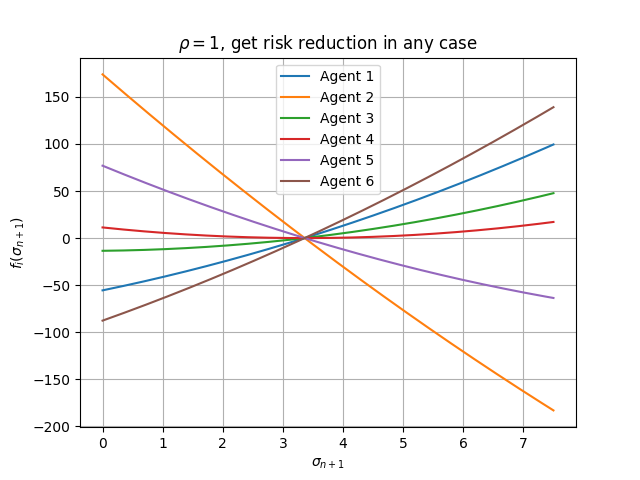
\includegraphics[width=0.6\textwidth]{Figures/Alwaysreduction.png}
\noindent\begin{minipage}{\textwidth}
\raggedright
\NOTE{\\{\it Note}: The parameters are $\rho=1$, $ \boldsymbol{\sigma}_6\approx(2.7, 12.6, 9, 20, 19.6, 0.2)$, $\boldsymbol{\delta}_{7}\approx(13.5, 7.1, 15.7, 19.2, 13, 7.2, 14.4)$.}
\end{minipage}
\label{fig:alwaysreduc}
\end{figure}

\subsection{Proofs of Section \ref{sec:equilibrium}}

\paragraph{Proof of Theorem \ref{thm:newpricing_mainthm_withoutsamecorr}}
\

Note that $\rho(Y_i^{(n)})\geq\rho(Y_i^{(n+1)})$
is equivalent to
$\rho(X_i)-\rho(Y_i^{(n)})\leq\rho(X_i)-\rho(Y_i^{(n+1)})$
and the result follows directly from \eqref{ineq:equi_stab_weak}.

% Given the risk-sharing rule of $n$ agents with the sharing ratio of each agent $i$ being $\lambda_{n,i}$, the entrance of the candidate benefits agent $i$, $i<n+1$, if and only if 
% \begin{align}\label{eq:entrance_newpricing_ex}
% \CE_i\left[\lambda_{n,i}S_n-\pi_{n,i}\right]\geq\CE_i\left[\lambda_{n+1,i}S_{n+1}-\pi_{n+1,i}\right].
% \end{align}
% From \eqref{eq:entrance_newpricing_ex},
% \begin{align*}
%     \CE_{i}[X_i]-\CE_i\left[\lambda_{n,i}S_n-\pi_{n,i}\right]\leq \CE_{i}[X_i]-\CE_i\left[\lambda_{n+1,i}S_{n+1}-\pi_{n+1,i}\right].
% \end{align*}
% By stability condition, it follows that
% \[
% \Var(X_i-\lambda_{n,i}S_n)\leq \Var(X_i-\lambda_{n+1,i}S_{n+1}).
% \]
% Equivalently,
% \begin{equation}\label{eq:Newpricing_strongineq}
%     -2\lambda_{n,i}\Cov(X_i,S_n)+ \lambda_{n,i}^2s^2_n\leq -2\lambda_{n+1,i}\Cov(X_i,S_{n+1})+ \lambda_{n+1,i}^2s^2_{n+1}.
% \end{equation}
% By rearranging with respect to $\rho_{n,n+1},$
% \[
% \rho_{n,n+1}\geq\frac{2\lambda_{n+1,i}\Cov(X_i,S_{n+1})-2\lambda_{n,i}\Cov(X_i,S_n)+ \lambda_{n,i}^2s^2_n-\lambda_{n+1,i}^2(\sigma_{n+1}^2+s_n^2)}{2\lambda_{n+1,i}^2\sigma_{n+1}s_n} 
% \]


\paragraph{Proof of Theorem \ref{thm:cases for agent i}} 
\

For the first item in the view to Table \ref{tab:table1}, we need to show that when $\sigma_i$ is sufficiently low for some $i=1,\cdots,n$, then $b_i^2\leq c_i$. Indeed, we calculate that $b_i^2\leq c_i$ is equivalent to 
\begin{align*}
2\left(\frac{\lambda_{n,i}-\lambda_{n+1,i}}{\lambda_{n+1,i}^2} -\frac{\lambda_{n,i}^2-\lambda_{n+1,i}^2}{\lambda_{n+1,i}^2}\right) & \sigma^2_i
+2\rho\sigma_i\Sigma^{(n)}_{-i}\left(\frac{\lambda_{n,i}-\lambda_{n+1,i}}{\lambda_{n+1,i}^2}-\frac{\lambda_{n,i}^2-\lambda_{n+1,i}^2}{\lambda_{n+1,i}^2}\right)\\    
&-\frac{\lambda_{n,i}^2-\lambda_{n+1,i}^2}{\lambda_{n+1,i}^2}s^2_{-i}\leq 0.
\end{align*}
Since $\lambda_{n,i}>\lambda_{n+1,i}$, the above holds when $\sigma_i$ is sufficiently low. 

As for the second item, we need to show for large $\sigma_i$ and $\rho$ we have $0\geq c_i<b_i^2$ and also $b_i>0$. Indeed, the latter holds exactly when $\sigma_i>\lambda_{n+1,i}\Sigma_{-i}^{(n)}/(1-\lambda_{n+1,i})$. For the former is equivalent to $f_i(b_i)\leq 0$. Note that  
$f_i(b_i)$ is a quadratic function of $\sigma_i$ with the coefficient of $\sigma_i^2$ equal to 
\[2\frac{\lambda_{n,i}-\lambda_{n+1,i}}{\lambda_{n+1,i}^2}-\frac{\lambda^2_{n,i}-\lambda^2_{n+1,i}}{\lambda_{n+1,i}^2}-\rho^2\frac{(1-\lambda_{n+1,i})^2}{\lambda_{n+1,i}^2}, \]
which is negative if and only if 
\[\rho^2>\frac{(\lambda_{n,i}-\lambda_{n+1,i})(2-(\lambda_{n,i}+\lambda_{n+1,i}))}{(1-\lambda_{n+1,i})^2}.\]
Hence, when both $\rho$ and $\sigma_i$ are sufficiently large, function $f_i(x)$ is positive at zero, becomes negative for a positive $x^*$ and then increases. This behavior is consistent with the statement.  

Finally, for the third item it is enough to show that $f_i(b_i)\geq 0$. $f_i(b_i)$ is a quadratic function of $\sigma_i$, the coefficient of $\sigma_i^2$ becomes positive when 
\[\rho^2<\frac{(\lambda_{n,i}-\lambda_{n+1,i})(2-(\lambda_{n,i}+\lambda_{n+1,i}))}{(1-\lambda_{n+1,i})^2}.\]
The above means that for sufficiently large $\sigma_i$ and when $\rho$ satisfies the above inequality, function $f_i(b_i)$ is always above zero and hence agent $i$ always accept the candidate. 
\bigskip

\paragraph{Proof of Corollary \ref{cor:equistrong_prop4}}
\

Note that
{\small
\[
\lim_{\rho\to1}f_i(\sigma_{n+1}|\,\boldsymbol{\sigma})=\sigma_{n+1}^2+2\left(\Sigma_{n}-(n+1)\sigma_i\right)\sigma_{n+1}+\frac{2n+2}{n}\left(\sigma_i^2+\sigma_i\sum_{j\neq i}^{n}\sigma_j\right)-\frac{2n+1}{n^2}\left(\sum_{j=1}^n\sigma_j^2+2\sum_{j\neq k}^{n}\sigma_j\sigma_k\right).
\]
}
The minimum is achieved at
\[
\frac{\partial}{\partial \sigma_{n+1}} \lim_{\rho\to1}f_i(\sigma_{n+1}|\,\boldsymbol{\sigma})=2\sigma_{n+1}+2(\Sigma_{n}-(n+1)\sigma_i)=0.
\]
Thus, $\sigma_{n+1}^*=(n+1)\sigma_i-\Sigma_n.$ First, suppose that $(n+1)\sigma_i-\Sigma_n<0$. Since the minimum is achieved when $\sigma_{n+1}<0,$ it suffices to prove that $f_i(\sigma_{n+1}=0|\boldsymbol{\sigma})<0.$ Define $\Sigma_{n-i}:=\sum_{j\neq i}^n\sigma_j.$ Then,
\begin{align*}
\lim_{\rho\to1}f_i(\sigma_{n+1}=0|\boldsymbol{\sigma})&=\frac{2n+2}{n}\left(\sigma_i^2+\sigma_i\sum_{j\neq i}^{n}\sigma_j\right)-\frac{2n+1}{n^2}\left(\sum_{j=1}^n\sigma_j^2+2\sum_{j\neq k}^{n}\sigma_j\sigma_k\right)\\
&=\frac{1}{n^2}\left((2n^2-1)\sigma_i^2+2(n^2-n-1)\sigma_i\Sigma_{n-i}-(2n+1)\Sigma_{n-i}^2\right)\\
&=(\sigma_i+\Sigma_{n-i})((2n^2-1)\sigma_i-(2n+1)\Sigma_{n-i})\\
&<0,
\end{align*}
where the last inequality comes from the imposed assumption.

Second, suppose that $(n+1)\sigma_i-\Sigma_n>0$. Since the minimum is achieved when $\sigma_{n+1}>0,$ we have to prove that $f_i(\sigma_{n+1}=\sigma_{n+1}^*|\boldsymbol{\sigma})<0.$ Note the minimum value is
{\small
\begin{align*}
\lim_{\rho\to1}f_i(\sigma_{n+1}|\,\boldsymbol{\sigma})|_{\sigma_{n+1}=\sigma_{n+1}^*}&=-((n+1)\sigma_i-\Sigma_n)^2+\frac{2n+2}{n}\left(\sigma_i^2+\sigma_i\sum_{j\neq i}^{n}\sigma_j\right)-\frac{2n+1}{n^2}\left(\sum_{j=1}^n\sigma_j^2+2\sum_{j\neq k}^{n}\sigma_j\sigma_k\right)\\
&=-\frac{1}{n^2}\left((n^2-1)^2\sigma_i^2-2(n-1)(n+1)^2\sigma_i\Sigma_{n-i}+(n+1)^2\Sigma_{n-i}^2\right)\\
&=-\frac{1}{n^2}(1+n)^2(\sigma_i-n\sigma_i+\Sigma_{n-i})^2\\
&<0,
\end{align*}
}
which completes the proof.
\bigskip

\paragraph{Proof of Theorem \ref{thm:strong consensus equilibrium 1}}
\

The first item follows directly since $f_i(\sigma_{n+1}|\,\boldsymbol{\sigma})$  is a quadratic function with a positive constant at the quadratic term. Thus, it is positive for sufficiently large $\sigma_{n+1}$ for all $i$ in any case.

For the second item, if $\sigma_{n+1}$ is sufficiently low, the strong consensus condition is determined by the by the existing member with the lower of $f_i$. For this, we consider two existing members $i,j$ and compare the limiting behavior of $f_i$ and $f_j$ when $\sigma_{n+1}$ goes to zero. We calculate that 
\begin{align*}
\lim_{\sigma_{n+1}\to0}[f_i(\sigma_{n+1})-f_j(\sigma_{n+1})]&= 2\frac{\delta_{n+1}\Delta_{n+1}}{\Delta_{n}}  \left(\frac{\sigma_i}{\delta_i}(\sigma_i-\rho\Sigma_{-i})- \frac{\sigma_j}{\delta_j}(\sigma_j-\rho\Sigma_{-j})\right),
\end{align*} 
where we have used the fact that $\lambda_{n,i}^2/\lambda_{n+1,i}^2$ does not depend on $i$. The above is negative if and only if 
\begin{align*}
\frac{\sigma^2_i}{\delta_i}-\frac{\sigma_j^2}{\delta_j} +\rho\frac{\sigma_i}{\delta_i}\frac{\sigma_j}{\delta_j}(\delta_j-\delta_i)  + \rho\Sigma_{-i,j}  \left(\frac{\sigma_i}{\delta_i}-\frac{\sigma_j}{\delta_j} \right)<0,
\end{align*}
where $\Sigma_{-i,j}:=\sum_{k\neq i,j}^n\sigma_k$. Thus, we may conclude that the existing member with sufficiently low risk and sufficiently high risk tolerance (that is sufficiently low deviation-tolerance ratio) determines the strong consensus condition. 

For the third item, we analogously examine the sign of the difference $f_i(\sigma_{n+1})-f_j(\sigma_{n+1})$ when $\sigma_{n+1}$ is sufficiently large. After simple calculations we get that this difference is negative if 
\[   \Delta_{n+1}\left(\frac{\sigma_j}{\delta_j}-\frac{\sigma_i}{\delta_i} \right)<0. 
\]
Thus for sufficiently large $\sigma_{n+1}$, the existing member with the higher deviation-tolerance ratio.

\paragraph{Proof of Theorem \ref{thm:common sigma}}
\

Imposing common variances $\sigma_i=\sigma $ and common risk tolerances $\delta_i=\delta$ for each $i=1,2,...,n$, \eqref{eq:withsamecor} becomes
% \[
% \sigma_{n+1}^2-2\rho\sigma\sigma_{n+1}+2\left(\frac{(n+1)^2}{n}-(n+1)\right)(\sigma^2+n\rho\sigma^2)-\left(\frac{2n+1}{n^2}\right)\left(n+\frac{n(n-1)}{2}\rho\right)\sigma^2\geq 0,
% \]
\[
\sigma_{n+1}^2-2\rho\sigma\sigma_{n+1}+\frac{2(n+1)(1+(n-1)\rho)}{n}\sigma^2-\frac{(2n+1)(1+(n-1)\rho)}{n}\sigma^2\geq 0,
\]
which reduces to
% \[
% \sigma_{n+1}^2-2\rho\sigma\sigma_{n+1}+\frac{\sigma^2}{n}+\sigma^2\rho\left(\frac{2n^2+n+1}{2n}\right)\geq 0.
% \]
\[
\sigma_{n+1}^2-2\rho\sigma\sigma_{n+1}+\frac{(1+(n-1)\rho)}{n}\sigma^2\geq 0,
\]
This is quadratic convex function of $\sigma_{n+1}$. Then, note that
\[
(\rho\sigma)^2-\frac{(1+(n-1)\rho)}{n}\sigma^2<0,
\]
if $(\rho-1)(n\rho+1)<0$. This condition holds for $-1/n<\rho<1$, {\it i.e.} when $\rho$ is positive or not too negative, which in turn implies that there is no real root for $\rho>0$. Thus all existing members get benefited by the candidate's entrance.

On the other hand, imposing only common variances simplifies function $f_i$ as below:
\begin{align*}
f_i(\sigma_{n+1}|\,\rho,\sigma,\boldsymbol{\delta}) &=\sigma_{n+1}^2+2 \frac{\sigma\rho}{\lambda_{n+1,i}} \left(n\lambda_{n+1,i}-1\right)\sigma_{n+1}\\
&+2\left(\frac{\lambda_{n,i}-\lambda_{n+1,i}}{\lambda_{n+1,i}^2}\right)\sigma^2\left(1+\rho(n-1)\right)-\frac{\lambda_{n,i}^2-\lambda_{n+1,i}^2}{\lambda_{n+1,i}^2}\sigma^2n\left(1+\rho(n-1) \right).
\end{align*}
The necessary condition for $A=\mathbb{R}_+$ for all $\delta_{n+1}$ is 
\[
f_i(0) = \sigma^2(1 + \rho(n - 1)) \frac{\lambda_{n,i} - \lambda_{n+1,i}}{\lambda_{n+1,i}^2} \left[ 2 - n(\lambda_{n,i} + \lambda_{n+1,i}) \right]>0,
\]
which becomes equivalent to $\lambda_{n,i}+\lambda_{n+1,i}<(2/n)$ for $n>1$. We then need $b_i\leq 0$ or $f_i(b_i)=f_i(0)-b_i^2\geq 0$ for each $i=1,2,...,n$. Since
\[
b_i = -\frac{\sigma \rho}{\lambda_{n+1,i}} (n\lambda_{n+1,i} - 1),
\]
the former means that $1/n<\lambda_{n+1,i}$, which cannot hold for all $i$. Hence, there is at least one existing member for which $f_i(b_i)=f_i(0)-b_i^2\geq 0$. However, taking $\delta_{n+1}\to0$ gives
\[
f_i(b_i) \to -\frac{\sigma^2 \rho^2}{\lambda_{n,i}^2}(n\lambda_{n,i} - 1)^2 < 0,
\quad \text{if } \lambda_{n,i} \neq \frac{1}{n},
\]
which proves the desired result.

As for the last part of the statement the following example (pictured in Figure \ref{fig:common}) provides the mentioned possibility. Consider $n=6$, $\rho\approx0.96$, common $\sigma=1$, and $\boldsymbol{\delta}_{n+1}\approx(6.4, 7.1,   6.2, 6.4, 6.8, 6.8, 8.4)$. 
\begin{figure}[t]
\caption{Three distinct acceptance region when common $\sigma.$ Green shaded regions consist the acceptance region.}
\centering
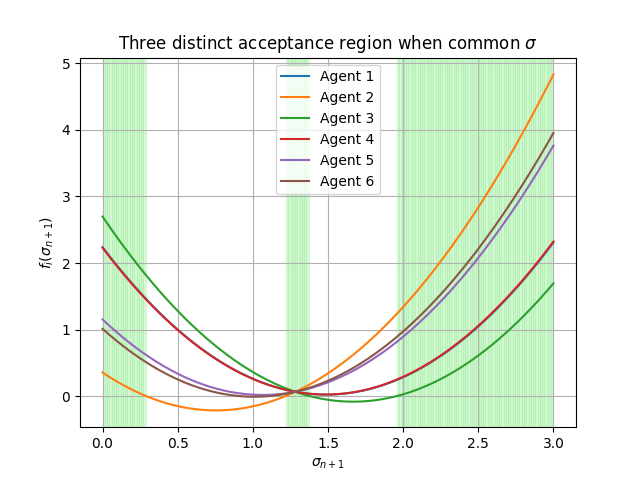
\includegraphics[width=0.6\textwidth]{Figures/common.png}
\label{fig:common}
\end{figure}

\paragraph{Proof of Theorem \ref{thm:common tolerance}}
\


When existing members' risk tolerances are fixed equal to $\delta$, \eqref{eq:entrance with new} becomes 
{\small
\[f_i(\sigma_{n+1}|\,\boldsymbol{\sigma}):=\sigma_{n+1}^2+2\rho\left(\Sigma_{n}-(n+1)\sigma_i\right)\sigma_{n+1}+\frac{2n+2}{n}\left(\sigma_i^2+\rho\sigma_i\sum_{j\neq i}^{n}\sigma_j\right)-\frac{2n+1}{n^2}\left(\sum_{j=1}^n\sigma_j^2+2\rho\sum_{j\neq k}^{n}\sigma_j\sigma_k\right),
\]
}
where $\boldsymbol{\sigma}=(\sigma_i)_{i=1,...,n}$. We prove the argument by proving an example of $n=2$ and assuming that $\delta_1=\delta_2=\delta_3$. We directly calculate that 
\begin{align*} 
f_1(x|\,\rho,\boldsymbol{\sigma}) &=x^2+2\rho\left(\sigma_{2}-2\sigma_1\right)x+3\left(\sigma_1^2+\rho\sigma_1\sigma_2\right)-\frac{5}{4}(\sigma_1^2+\sigma_2^2+2\rho\sigma_1\sigma_2)\\
f_2(x|\,\rho,\boldsymbol{\sigma}) &=x^2+2\rho\left(\sigma_{1}-2\sigma_2\right)x+3\left(\sigma_2^2+\rho\sigma_1\sigma_2\right)-\frac{5}{4}(\sigma_1^2+\sigma_2^2+2\rho\sigma_1\sigma_2).
\end{align*}
Assuming without loss of generality $\sigma_1<\sigma_2$. This directly implies that $b_1<b_2$. We will show that there is a combination of inputs $\sigma_1,\sigma_2$ and $\rho$ for which 
\[A=[0,b_1-\sqrt{c_1}]\cup[b_1+\sqrt{c_1},b_2-\sqrt{c_2}]\cup[b_2-\sqrt{c_2},\infty). \]
Based on the Table \ref{tab:table1}, we get that the following form of $A$ occurs when $0<b_1$, $0<f_1(0)$, $f_2(b_2)<0$ and $b_1+\sqrt{c_1}<b_2-\sqrt{c_2}$. The first requirement is equivalent with the inequality $\sigma_2<2\sigma_1$. On the other hand, if $f_1(0)>0$ then we also have that $f_2(0)>0$ (since $\sigma_1<\sigma_2$). The former is equivalent to  
\[7\sigma_1^2-5\sigma_2^2+2\rho\sigma_1\sigma_2>0.\]
The above holds for all $\sigma_1>\sigma_2(\sqrt{\rho^2+35}-\rho)/7$. Note that this inequality is consistent with the $\sigma_1<\sigma_2<2\sigma_1$. The inequality $f_2(b_2)<0$ is equivalent to 
\[\sigma_2^2\frac{7-16\rho^2}{4}-\sigma_1^2\frac{5+4\rho^2}{4}+\sigma_1\sigma_2\rho(4\rho-3)\leq 0.\]
The above is decreasing in $\rho$ and has a unique root in $\hat{\rho}\in[0,1]$, at which and above the inequality holds. Finally, 
$b_1+\sqrt{c_1}<b_2-\sqrt{c_2}$ is equivalent to 
\[\sqrt{-f_1(b_1)}+\sqrt{-f_2(b_2)}<3\rho(\sigma_2-\sigma_1). \]


% \subsection{Proof: Proposition \ref{prop:equistrong_prop8}}
% example for more than two intervals when the risk tolerances are different: $\boldsymbol{\sigma}=(2,1,8,8,\sigma_{n+1}),$ $\boldsymbol{\delta}=(0.95923546, 1.03989315, 3.72922139, 3.72523192, 2.9135696),$ $\rho=0.5269359793514463.$ This has three areas of acceptance, $\sigma_{n+1}\in(0,1.5)\cup(2.5,3.3)\cup(7.4,\infty).$ \textcolor{red}{need proof or counterexample for common risk tolerance case}

\section{Supplementary Materials for Section \ref{sec:Equilibrium with Reinsurance}}\label{App:D}

\subsection{Analytic expression for SC with reinsurance EP}\label{subsec:analytic expressions}

We give the analytic formulas for the inequality's components  $\EE[e^{\bar{S}_n/\Delta_n}]$, $\bar{\EE}_n[X_i]$, $\bar{\EE}_n[S_n]$, and $\EE[(S_n-K_n)_+]$.

\noindent 1. We have known formula for the moment generating function of the truncated normal random variable. That gives
\begin{align*}
\EE[e^{\bar{S}_n/\Delta_n}]&=\mathbb{E}\left[e^{S_n/\Delta_n}|S_n<K_n\right]\mathbb{P}[S_n<K_n]+\mathbb{E}\left[e^{K_n/\Delta_n}|S_n\geq K_n\right]\mathbb{P}[S_n\geq K_n]\\
&=\left(e^{\frac{1}{\Delta_{n}}m_n+\frac{1}{2\Delta_{n}^2}s_{n}^2}\right)\Phi\left(\beta-\frac{1}{\Delta_{n}}s_{n}\right)+e^{(m_n+s_n\beta)/\Delta_n}(1-\Phi(\beta)).
\end{align*}
2. We already have the denominator, $\ex{e^{\Bar{S}_n/\Delta_n}}$, so we only solve for the numerator. Note that
\begin{align*}
\EE[X_i e^{\bar{S}_n/\Delta_n}]&=\EE[X_i e^{\bar{S}_n/\Delta_n}\mathbbm{1}_{\{S_n\leq K_n\}}]+\EE[X_i e^{\bar{S}_n/\Delta_n}\mathbbm{1}_{\{S_n>K_n\}}].
\end{align*}
Define $A_n:=K_n-\sum_{j\neq i}^nX_j\sim\Normal(\mu_a,\sigma_a^2)$. Note that
\[
\EE[X_i e^{\bar{S}_n/\Delta_n}\mathbbm{1}_{\{S_n>K_n\}}]=e^{K_n/\Delta_n}\EE[X_i\mathbbm{1}_{\{S_n>K_n\}}]=e^{K_n/\Delta_n}\EE[X_i\mathbbm{1}_{\{X_i>A_n\}}].
\]
By the law of total expectation,
\[
\ex{X_i\mathbbm{1}_{\{X_i\geq A_n\}}}=\ex{\ex{X_i\mathbbm{1}_{\{X_i\geq A_n\}}|X_i}}.
\]
Evaluating the expectation,
\[
\ex{X_i\mathbbm{1}_{\{X_i\geq A_n\}}|X_i}=\int_{-\infty}^{\infty}x_i\mathbbm{1}_{\{x_i\geq A_n\}}f_{X_i}(x_i)dx_i=\int_{A_n}^{\infty}x_if_{X_i}(x_i)dx_i.
\]
Then,
\begin{align*}
\int_{A_n}^{\infty}x_if_{X_i}(x_i)dx_i&=-\frac{\sigma_i}{\sqrt{2\pi}}\int_{A_n}^{\infty}-\frac{x_i-\mu_i}{\sigma_i^2}e^{-\frac{(x_i-\mu_i)^2}{2\sigma_i^2}}dx_i+\frac{\mu_i}{\sqrt{2\pi}\sigma_i}\int_{A_n}^{\infty}e^{-\frac{(x_i-\mu_i)^2}{2\sigma_i^2}}dx_i\\
&=\frac{\sigma_i}{\sqrt{2\pi}}e^{-\frac{(A_n-\mu_i)^2}{2\sigma_i^2}}+\mu_i\prob{X_i\geq A_n}=\frac{\sigma_i}{\sqrt{2\pi}}e^{-\frac{(A_n-\mu_i)^2}{2\sigma_i^2}}+\mu_i\prob{S_n\geq K_n}\\
&=\frac{\sigma_i}{\sqrt{2\pi}}e^{-\frac{(A_n-\mu_i)^2}{2\sigma_i^2}}+\mu_i(1-\Phi(\beta))
\end{align*}
Thus,
\begin{align*}
\ex{\ex{X_i\mathbbm{1}_{\{X_i\geq A_n\}}|X_i}}
&=\ex{\frac{\sigma_i}{\sqrt{2\pi}}e^{-\frac{(A_n-\mu_i)^2}{2\sigma_i^2}}}+\mu_i(1-\Phi(\beta)).
\end{align*}
For the first term,
\begin{align*}
\ex{e^{-\frac{(A_n-\mu_i)^2}{2\sigma_i^2}}}&=\int_{-\infty}^{\infty}e^{-\frac{(a_n-\mu_i)^2}{2\sigma_i^2}}\frac{1}{\sqrt{2\pi}\sigma_{a}}e^{-\frac{(a_n-\mu_a)^2}{2\sigma_a^2}}da_n\\
&=\frac{e^{-\frac{1}{2}\left(\frac{\mu_i^2\sigma_a^2+\sigma_i^2\mu_a^2}{\sigma_i^2\sigma_a^2}-\frac{\left(\mu_i^2\sigma_a^2+\sigma_i^2\mu_a^2\right)^2}{\sigma_a^2\sigma_i^2(\sigma_a^2+\sigma_i^2)}\right)}}{\sqrt{2\pi}\sigma_{a}}\int_{-\infty}^{\infty}e^{-\frac{1}{2}\frac{\left(a_n-\frac{\left(\mu_i^2\sigma_a^2+\sigma_i^2\mu_a^2\right)^2}{\sigma_a^2\sigma_i^2(\sigma_a^2+\sigma_i^2)}\right)^2}{\frac{\sigma_i^2\sigma_a^2}{\sigma_a^2+\sigma_i^2}}}d a_n\\
&=\frac{e^{-\frac{1}{2}\left(\frac{\mu_i^2\sigma_a^2+\sigma_i^2\mu_a^2}{\sigma_i^2\sigma_a^2}-\frac{\left(\mu_i^2\sigma_a^2+\sigma_i^2\mu_a^2\right)^2}{\sigma_a^2\sigma_i^2(\sigma_a^2+\sigma_i^2)}\right)}}{\sqrt{2\pi}\sigma_{a}}\sqrt{2\pi\frac{\sigma_i^2\sigma_a^2}{\sigma_a^2+\sigma_i^2}}\\
&=\frac{\sigma_ie^{-\frac{1}{2}\left(\frac{\mu_i^2\sigma_a^2+\sigma_i^2\mu_a^2}{\sigma_i^2\sigma_a^2}-\frac{\left(\mu_i^2\sigma_a^2+\sigma_i^2\mu_a^2\right)^2}{\sigma_a^2\sigma_i^2(\sigma_a^2+\sigma_i^2)}\right)}}{\sqrt{\sigma_a^2+\sigma_i^2}}
\end{align*}
Therefore,
\begin{align*}
\ex{X_i\mathbbm{1}_{\{X_i\geq A_n\}}}=\frac{\sigma_i^2e^{-\frac{1}{2}\left(\frac{\mu_i^2\sigma_a^2+\sigma_i^2\mu_a^2}{\sigma_i^2\sigma_a^2}-\frac{\left(\mu_i^2\sigma_a^2+\sigma_i^2\mu_a^2\right)^2}{\sigma_a^2\sigma_i^2(\sigma_a^2+\sigma_i^2)}\right)}}{\sqrt{2\pi(\sigma_a^2+\sigma_i^2)}}+\mu_i(1-\Phi(\beta)).
\end{align*}

Then,
\begin{align*}
\EE[X_i e^{\bar{S}_n/\Delta_n}\mathbbm{1}_{\{S_n\leq K_n\}}]&=\mathbb{E}\left[X_ie^{S_n/\Delta_n}|S_n<K_n\right]\mathbb{P}[S_n<K_n]\\
&=\mathbb{E}\left[X_ie^{S_n/\Delta_n}|S_n<K_n\right]\Phi(\beta)
\end{align*}
Let $\tb{X}=(X_1,X_2,...,X_n)\sim\Normal(\boldsymbol{\mu},\boldsymbol{\Sigma})$. Then, $\tb{t}^\top\tb{X}\sim\Normal(\tb{t}^\top\boldsymbol{\mu},\tb{t}^\top\boldsymbol{\Sigma}\tb{t}).$ We know that
\[
\mathbb{E}\left[e^{\tb{t}^\top\tb{X}}|\tb{t}^\top\tb{X}<K_n\right]=e^{\tb{t}^\top\boldsymbol{\mu}+\tb{t}^\top\boldsymbol{\Sigma}\tb{t}/2}\frac{\Phi\left(\frac{K_n-\tb{t}^\top\boldsymbol{\mu}}{\sqrt{\tb{t}^\top\boldsymbol{\Sigma}\tb{t}}}-\sqrt{\tb{t}^\top\boldsymbol{\Sigma}\tb{t}}\right)}{\Phi\left(\frac{K_n-\tb{t}^\top\boldsymbol{\mu}}{\sqrt{\tb{t}^\top\boldsymbol{\Sigma}\tb{t}}}\right)}.
\]
Taking the derivative with respect to $t_i$ gives 
{\small \begin{align*}
&\mathbb{E}\left[X_ie^{\tb{t}^\top\tb{X}}|\tb{t}^\top\tb{X}<K_n\right]=\left(\mu_i+\sum_{j=1}^nt_j\Cov(X_i,X_j)\right)e^{\tb{t}^\top\boldsymbol{\mu}+\tb{t}^\top\boldsymbol{\Sigma}\tb{t}/2}\frac{\Phi\left(\frac{K_n-\tb{t}^\top\boldsymbol{\mu}}{\sqrt{\tb{t}^\top\boldsymbol{\Sigma}\tb{t}}}-\sqrt{\tb{t}^\top\boldsymbol{\Sigma}\tb{t}}\right)}{\Phi\left(\frac{K_n-\tb{t}^\top\boldsymbol{\mu}}{\sqrt{\tb{t}^\top\boldsymbol{\Sigma}\tb{t}}}\right)}\\
&+e^{\tb{t}^\top\boldsymbol{\mu}+\tb{t}^\top\boldsymbol{\Sigma}\tb{t}/2}\left(\frac{-\mu_i(\tb{t}^\top\boldsymbol{\Sigma}\tb{t})-(K_n-\tb{t}^\top\boldsymbol{\mu})\sum_{j= 1}^nt_j\Cov(X_i,X_j)}{\left(\tb{t}^\top\boldsymbol{\Sigma}\tb{t}\right)^{3/2}}-\frac{\sum_{j= 1}^nt_j\Cov(X_i,X_j)}{2\sqrt{\tb{t}^\top\boldsymbol{\Sigma}\tb{t}}}\right)\frac{\phi\left(\frac{K_n-\tb{t}^\top\boldsymbol{\mu}}{\sqrt{\tb{t}^\top\boldsymbol{\Sigma}\tb{t}}}-\sqrt{\tb{t}^\top\boldsymbol{\Sigma}\tb{t}}\right)}{\Phi\left(\frac{K_n-\tb{t}^\top\boldsymbol{\mu}}{\sqrt{\tb{t}^\top\boldsymbol{\Sigma}\tb{t}}}\right)}\\
&+e^{\tb{t}^\top\boldsymbol{\mu}+\tb{t}^\top\boldsymbol{\Sigma}\tb{t}/2}\Phi\left(\frac{K_n-\tb{t}^\top\boldsymbol{\mu}}{\sqrt{\tb{t}^\top\boldsymbol{\Sigma}\tb{t}}}-\sqrt{\tb{t}^\top\boldsymbol{\Sigma}\tb{t}}\right)\left(\frac{-\mu_i(\tb{t}^\top\boldsymbol{\Sigma}\tb{t})-(K_n-\tb{t}^\top\boldsymbol{\mu})\sum_{j= 1}^nt_j\Cov(X_i,X_j)}{\left(\tb{t}^\top\boldsymbol{\Sigma}\tb{t}\right)^{3/2}}\right)\frac{\phi\left(\frac{K_n-\tb{t}^\top\boldsymbol{\mu}}{\sqrt{\tb{t}^\top\boldsymbol{\Sigma}\tb{t}}}\right)}{\left(\Phi\left(\frac{K_n-\tb{t}^\top\boldsymbol{\mu}}{\sqrt{\tb{t}^\top\boldsymbol{\Sigma}\tb{t}}}\right)\right)^2}
\end{align*}
}
Taking $\tb{t}^*$ be the vector of ones gives $(\tb{t}^*)^\top\tb{X}=S_n\sim\Normal(m_n,s_n^2).$ 
% Thus, it follows that
% \begin{align*}
%     \mathbb{E}&\left[X_ie^{S_n}|S_n<K_n\right]=\left(\mu_i+\sum_{j=1}^n\Cov(X_i,X_j)\right)e^{m_n+s_n^2/2}\frac{\Phi\left(\frac{K_n-m_n}{s_n}-s_n\right)}{\Phi\left(\frac{K_n-m_n}{s_n}\right)}\\
%     &+e^{m_n+s_n^2/2}\left(\frac{-\mu_is_n^2-(K_n-m_n)\sum_{j= 1}^n\Cov(X_i,X_j)}{s_n^{3/2}}-\frac{\sum_{j= 1}^n\Cov(X_i,X_j)}{2s_n}\right)\frac{\phi\left(\frac{K_n-m_n}{s_n}-s_n\right)}{\Phi\left(\frac{K_n-m_n}{s_n}\right)}\\
%     &+e^{m_n+s_n^2/2}\Phi\left(\frac{K_n-m_n}{s_n}-s_n\right)\left(\frac{-\mu_is_n-(K_n-m_n)\sum_{j= 1}^n\Cov(X_i,X_j)}{\left(s_n\right)^{3/2}}\right)\frac{\phi\left(\frac{K_n-m_n}{s_n}\right)}{\left(\Phi\left(\frac{K_n-m_n}{s_n}\right)\right)^2}
% \end{align*}
Since $K_n=m_n+\beta s_n,$
\begin{align*}
\mathbb{E}&\left[X_ie^{S_n}|S_n<K_n\right]=\left(\mu_i+\sum_{j=1}^n\Cov(X_i,X_j)\right)e^{m_n+s_n^2/2}\frac{\Phi\left(\beta-s_n\right)}{\Phi\left(\beta\right)}\\
&+e^{m_n+s_n^2/2}\left(\frac{-\mu_is_n-s_n\beta\sum_{j= 1}^n\Cov(X_i,X_j)}{s_n^{1/2}}-\frac{\sum_{j= 1}^n\Cov(X_i,X_j)}{2s_n}\right)\frac{\phi\left(\beta-s_n\right)}{\Phi\left(\beta\right)}\\
&+e^{m_n+s_n^2/2}\Phi\left(\beta-s_n\right)\left(\frac{-\mu_i-\beta\sum_{j= 1}^n\Cov(X_i,X_j)}{\left(s_n\right)^{1/2}}\right)\frac{\phi\left(\beta\right)}{\left(\Phi\left(\beta\right)\right)^2}
\end{align*}
Similarly, taking $\tb{t}^*$ be the vector of ones divided by $\Delta_n$ gives $(\tb{t}^*)^\top\tb{X}=S_n/\Delta_n.$ This gives the desired expression.
\medskip


\noindent 3. We have
\begin{align*}
\bar{\EE}_n[S_n]&=\frac{\EE[S_n e^{\bar{S}_n/\Delta_n}]}{\EE[e^{\bar{S}_n/\Delta_n}]},
\end{align*}
where
\begin{align*}
\EE[S_n e^{\bar{S}_n/\Delta_n}]&=\mathbb{E}\left[S_ne^{S_n/\Delta_n}|S_n<K_n\right]\mathbb{P}[S_n<K_n]+\mathbb{E}\left[S_ne^{K_n/\Delta_n}|S_n\geq K_n\right]\mathbb{P}[S_n\geq K_n].
\end{align*}
All other things are known except $\mathbb{E}\left[S_ne^{S_n/\Delta_n}|S_n<K_n\right].$ Note that for the normal random variable $X\sim \Normal(\mu,\sigma^2),$ the moment generating function of its truncation $X<b$ is given by
\[
\mathbb{E}\left[e^{tX}|X<b\right]=e^{\mu t+\sigma^2t^2/2}\frac{\Phi\left(\frac{b-\mu}{\sigma}-\sigma t\right)}{\Phi\left(\frac{b-\mu}{\sigma}\right)}.
\]
Taking a derivative on both sides with respect to $t$ gives
\[
\mathbb{E}\left[Xe^{tX}|X<b\right]=\frac{e^{\mu t+\sigma^2t^2/2}}{\Phi\left(\frac{b-\mu}{\sigma}\right)}\left((\mu +\sigma^2t)\Phi\left(\frac{b-\mu}{\sigma}-\sigma t\right)-\sigma \phi\left(\frac{b-\mu}{\sigma}-\sigma t\right)\right).
\]
This implies that
\begin{align*}
\mathbb{E}\left[S_ne^{S_n/\Delta_n}|S_n<K_n\right]&=\frac{e^{\frac{m_n}{\Delta_n}+\frac{s_n^2}{2\Delta_n^2}}}{\Phi\left(\beta\right)}\left(\left(m_n+\frac{s_n^2}{\Delta_n}\right)\Phi\left(\beta-\frac{s_n}{\Delta_n} \right)-s_n \phi\left(\beta-\frac{s_n}{\Delta_n}\right)\right).
\end{align*}
Therefore,
{\small
\begin{align*}
\bar{\EE}_n[S_n]&=\frac{e^{\frac{m_n}{\Delta_n}+\frac{s_n^2}{2\Delta_n^2}}\left(\left(m_n+\frac{s_n^2}{\Delta_n}\right)\Phi\left(\beta-\frac{s_n}{\Delta_n} \right)-s_n \phi\left(\beta-\frac{s_n}{\Delta_n}\right)\right)+e^{\frac{(m_n+s_n\beta)}{\Delta_n}}\left(m_n+\frac{s_n\phi(\beta)}{1-\Phi(\beta)}\right)(1-\Phi(\beta))}{\left(e^{\frac{1}{\Delta_{n}}m_n+\frac{1}{2\Delta_{n}^2}s_{n}^2}\right)\Phi\left(\beta-\frac{1}{\Delta_{n}}s_{n}\right)+e^{(m_n+s_n\beta)/\Delta_n}(1-\Phi(\beta))}
\end{align*}
}

\noindent 4.  Stop loss transformation has known formula.
\begin{align*}
\EE[(S_n-K_n)_+]&=\mathbb{E}\left[S_n-K_n|S_n\geq K_n\right]\mathbb{P}[S_n\geq K_n]\\
&=s_n\left(\phi(\beta)-\beta(1-\Phi(\beta))\right).
\end{align*}
Thus, we have the closed form formula for $
\rho_i(Y^{(n)}_i)\geq \rho_i(Y^{(n+1)}_i)$. 

\subsection{Example: the effect of reinsurance on the expansion under EP}\label{app:eg:EP_rein}
We present a simplified example that highlights the effect of reinsurance. Consider a risk pool with only two members, i.e. $n=2$ where $X_1\sim\Normal(5, 9)$, $X_2\sim\Normal(9, 169)$, $\rho_{X_1,X_2}=0.2$, $\delta_1=\delta_2=1$, and $K=25.4$  ($\beta=0.7125$). Observe that the second existing member has a much higher risk. We first consider the effect of reinsurance on existing members. We readily get that  
\[
\rho_1(\bar{Y}_2)\approx2.92\,>\,-2.87\approx\rho_1(Y_2),
\]
which means that the first member's position worsens due to the reinsurance. We have seen in Remark \ref{rem:gains from reinsurance} that the aggregate gain from the reinsurance is positive \textit{i.e.} $\rho_1(Y_2)+\rho_2(Y_2)>\rho_1(\bar{Y}_2)+\rho_2(\bar{Y}_2)$, which implies that the second member benefits from the reinsurance (as expected). How is the situation affected by a new entrance? Without reinsurance, the gain of the second agent from the pool's expansion is much higher than that of a first agent when $\sigma_{3}$ is large (see Figure \ref{fig:Equi_counter_wo_R}). With reinsurance, benefits from the pool's expansion are lower for both members, and acceptance regions (in terms of $\sigma_{3}$) become narrower for both members (see Figure \ref{fig:Equi_counter_w_R}). Comparing Figures \ref{fig:Equi_counter_wo_R} and \ref{fig:Equi_counter_w_R}, we note that the second agent no longer always accepts the candidate in the presence of reinsurance and that the first agent has a slightly higher requirement for the variance of the candidate. This example is consistent with the fact that reinsurance may reduce gains from a new entrance and hence existing members impose stricter requirements for accepting a candidate.
\begin{figure}[t]
\caption{Example \ref{app:eg:EP_rein}.}
\centering
\begin{subfigure}[b]{0.48\textwidth}
\centering
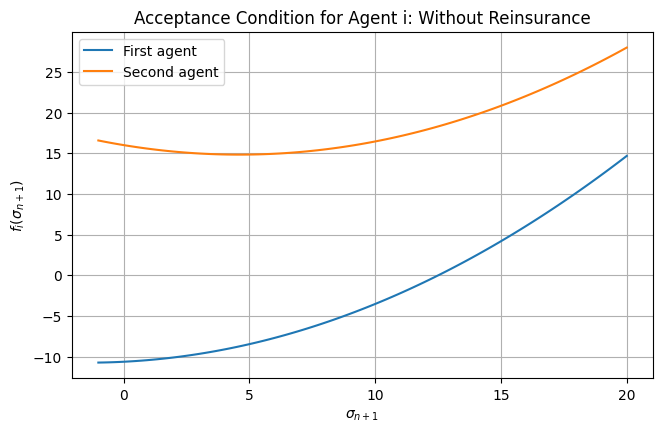
\includegraphics[width=\textwidth]{Figures/Equi_counter_wo_R.png}
\subcaption{}
\label{fig:Equi_counter_wo_R}
\end{subfigure}
\hfill
\begin{subfigure}[b]{0.48\textwidth}
\centering
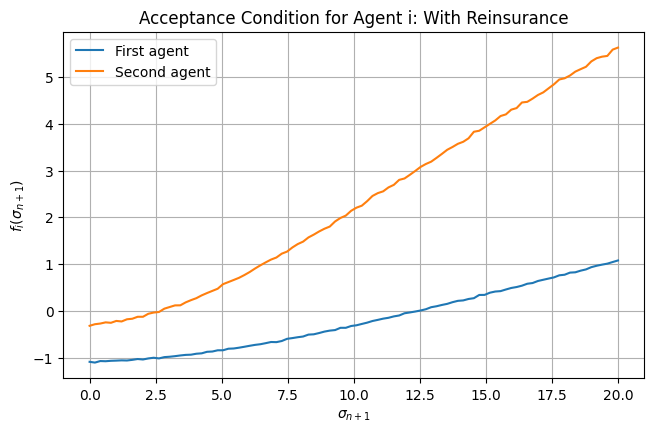
\includegraphics[width=\textwidth]{Figures/Equi_counter_w_R.png}
\subcaption{}
\label{fig:Equi_counter_w_R}
\end{subfigure}
\end{figure}


\subsection{Proofs of Section \ref{sec:Equilibrium with Reinsurance}}
\paragraph{Proof of Theorem \ref{thm:reinsurance cost}}
\

The following inequalities are equivalent:
\begin{align*}
\bar{\EE}[(S_n-K)_+]&\geq \EE[(S_n-K)_+]\\
\frac{\EE[(S_n-K)_+e^{\bar{S}_n/\Delta_{n}}]}{\EE[e^{\bar{S}_n/\Delta_{n}}]}&\geq \EE[(S_n-K)_+]\\
\EE[(S_n-K)_+e^{\bar{S}_n/\Delta_{n}}]& \geq \EE[(S_n-K)_+]\EE[e^{\bar{S}_n/\Delta_{n}}]\\
\EE[(S_n-K)_+e^{\bar{S}_n/\Delta_{n}}]& \geq \EE[(S_n-K)_+]\EE[e^{\bar{S}_n/\Delta_{n}}]\\
\Cov((S_n-K)_+,e^{\bar{S}_n/\Delta_{n}})& \geq 0.
\end{align*}
The latter always holds because $(S_n-K)_+$ and $e^{\bar{S}_n/\Delta_{n}}$ are non-decreasing functions of $S_n$. 

\bigskip

\paragraph{Proof of Theorem \ref{thm:reinsurance stability and weak consensus}}
\

For the stability we need to verify that the risk measure of each individual agent under risk-sharing with reinsurance is lower than the corresponding when he is outside the pool. This however comes from the definition of the demand function $\bar{z}_i^*$. Indeed, at equilibrium prices $(\tb{p}^*,\bar{p}^*)$, the optimal demand is different than zero and hence the participation in the equilibrium risk sharing is better than staying outside (which is equivalent to zero demand). Taking into account the fact that under the suggested cash transfer \eqref{eq:suggested payment} the payment is lower than that at the equilibrium we get the verification of the stability for each agent. 

The argument is similar for the weak consensus, since therein we compare the risk reduction inside a pool of $n+1$ agents and the staying outside of risk-sharing. 
\bigskip

\paragraph{Proof of 
Remark \ref{rem:gains from reinsurance}}
\

We need to show the following inequality:
\begin{equation}\label{inequality insurance}
\sum_{i=1}^n\rho_i(X_i+a^*\cdot X+a_i^*\cdot p^*)\geq \sum_{i=1}^n \rho_i(X_i+\bar{a}_i\cdot X +\bar{a}_i\bar{S}_n -\bar{a}_i\cdot \bar{p}^* -\bar{a}_i\bar{p})
\end{equation}
where the $(a^*,p^*)$ are the equilibrium allocation and prices without reinsurance and $(\bar{a},\bar{p})$ the corresponding quantities at the equilibrium with reinsurance at level $K$. From the calculation of both equilibria, we have that inequality is equivalent to 
\begin{equation}\label{inequality insurance2}
\Delta\log\left(\EE[e^{\bar{S}_n/\Delta}]\right)+\EE[(S_n-K)_+]\leq    \Delta\log\left(\EE[e^{S_n/\Delta}]\right). 
\end{equation}
This is equivalent to 
\begin{align*}
0 &\leq \log\left(\frac{\EE[e^{S_n/\Delta}]}{\EE[e^{\bar{S}_n/\Delta}]}\right)-\frac{1}{\Delta}\EE[(S_n-K)_+]\\   
1 &\leq \frac{\EE[e^{S_n/\Delta}]}{\EE[e^{\bar{S}_n/\Delta}]e^{\EE[(S_n-K)_+]/\Delta}}\\
& \EE[e^{\bar{S}_n/\Delta}]e^{\EE[(S_n-K)_+]/\Delta} \leq \EE[e^{S_n/\Delta}].
\end{align*}
By the Jensen inequality we have that $e^{\EE[(S_n-K)_+]/\Delta}\leq \EE[e^{(S_n-K)_+}/\Delta] $ and since $e^{(S_n-K)_+}$ and $e^{\bar{S}_n/\Delta}$ have positive Covariance (they are both monotonic to $S_n$), we have that 
\[\EE[e^{\bar{S}_n/\Delta}]e^{\EE[(S_n-K)_+]/\Delta}\leq \EE[e^{\bar{S}_n/\Delta}]\EE[e^{(S_n-K)_+/\Delta}]\leq \EE[e^{\bar{S}_n/\Delta}e^{(S_n-K)_+/\Delta}]= \EE[e^{S_n/\Delta}], \]
which completes the proof. 

\bigskip


\bibliography{bibliography}

\end{document} 


% Acknowledgments here
% \ACKNOWLEDGMENT{The authors are grateful to the associate editor and two anonymous referees for valuable comments on an earlier version of the paper. The research of the first author is supported by NWO Grant 613.001.208. The third author acknowledges the funding support from the Singapore Ministry of Education Social Science Research Thematic Grant MOE2016-SSRTG-059. Disclaimer: Any opinions, findings, and conclusions or recommendations expressed in this material are those of the author(s) and do not reflect the views of the Singapore Ministry of Education or the Singapore Government.}	

% \bibliography{bibliography}
% CASE 1: BiBTeX used to constantly update the references
%   (while the paper is being written).
%\bibliographystyle{ormsv080} % outcomment this and next line in Case 1
%\bibliography{<your bib file(s)>} % if more than one, comma separated

% CASE 2: BiBTeX used to generate mypaper.bbl (to be further fine tuned)
%\input{mypaper.bbl} % outcomment this line in Case 2

%If you don't use BiBTex, you can manually itemize references as shown below.

%\newpage

% \begin{thebibliography}{}%
% 			\bibitem[{Ardestani-Jaafari and Delage(2016a)}]{ad16a}
% 			Ardestani-Jaafari, A., E. Delage (2016a)
% 			Linearized robust counterparts of two-stage robust optimization problems with applications in operations management. Available at: { \url{optimization-online.org/DB_FILE/2016/03/5388.pdf}}.

% 			\bibitem[{Ardestani-Jaafari and Delage(2016b)}]{ad16b}
% 			Ardestani-Jaafari, A., E. Delage (2016b)
% 			Robust optimization of sums of piecewise linear functions with application to inventory problems.  {\it Operations Research} 64(2):474--494.

% 			\bibitem[{Bemporad et~al.(2003)}]{bbm03}
% 			Bemporad, A., F. Borrelli, M. Morari (2003)
% 			Min-max control of constrained uncertain discrete-time linear systems.
% 			{\it IEEE Transactions Automatic Control} 48(9):1600--1606.	

% 			\bibitem[{Ben-Ameur et~al.(2016)}]{bwoz16}
% 			Ben-Ameur, W., G. Wang, A. Ouorou, M. Zotkiewicz  (2016)
% 			Multipolar Robust Optimization. Available at: { \url{arxiv.org/pdf/1604.01813.pdf}}.	


% 			\bibitem[{Ben-Tal et~al.(2009)}]{ben09}
% 			Ben-Tal, A., L. El Ghaoui,   A. Nemirovski (2009)
% 			{\it Robust Optimization}.
% 			Princeton Series in Applied Mathematics (Princeton University Press, Princeton, NJ).

% 			\bibitem[{Ben-Tal et~al.(2015)}]{bdv15}
% 			Ben-Tal, A., D. den Hertog, J.P. Vial (2015)
% 			Deriving robust counterparts of nonlinear uncertain inequalities.
% 			{\it Mathematical Programming} 149(1):265--299.


% 			\bibitem[{Ben-Tal et~al.(2016)}]{beg16}
% 			Ben-Tal, A., O. El Housni, V. Goyal (2016)
% 			A tractable approach for designing piecewise affine policies in dynamic robust optimization. Available at: \url{optimization-online.org/DB_FILE/2016/07/5557.pdf}.


% 			\bibitem[{Ben-Tal et~al.(2004)}]{bggn04}
% 			Ben-Tal, A., A. Goryashko, E. Guslitzer, A. Nemirovski (2004)
% 			Ajustable robust solutions of uncertain linear programs. {\it Mathematical Programming} 99:351--376.

% 			\bibitem[{Ben-Tal and Nemirovski(1998)}]{bn98}
% 			Ben-Tal, A., A. Nemirovski (1998)
% 			Robust convex optimization. {\it Mathematics of Operations Research} 23(4):769--805.

% 			\bibitem[{Ben-Tal and Nemirovski(1999)}]{bn99}
% 			Ben-Tal, A., A. Nemirovski (1999)
% 			Robust solutions of uncertain linear programs. {\it Operations Research Letters} 25:1--13.

% 			\bibitem[{Ben-Tal and Nemirovski(2000)}]{bn00}
% 			Ben-Tal, A., A. Nemirovski (2000)
% 			Robust solutions of linear programming problems contaminated with uncertain data. {\it Mathematical Programming} 88(3):411--424.


% 			\bibitem[Bertsimas and Brown(2009)]{bb09}
% 			Bertsimas, D., D. Brown (2009)
% 			Constructing uncertainty sets for robust linear optimization. {\it Operations Research} 57(6):1483--1495.

% 			\bibitem[Bertsimas et~al.(2011)]{bbc11}
% 			Bertsimas, D.,  D. Brown,  C. Caramanis (2011).
% 			Theory and applications of robust optimization. {\it SIAM Review}, 53(3):464--501.


% 			\bibitem[Bertsimas and Caramanis(2010)]{bc10}
% 			Bertsimas, D.,   C. Caramanis (2010).
% 			Finite adaptability for linear optimization. {\it IEEE Transactions on Automatic Control}, 55(12):1751--2766.

% 			\bibitem[{Bertsimas and Dunning(2016)}]{bd16a}
% 			Bertsimas, D., I. Dunning (2016)
% 			Multistage robust mixed integer optimization with adaptive partitions.  {\it Operations Research} 64(4):980--998.

% 			\bibitem[{Bertsimas et~al.(2015)}]{bdl15}
% 			Bertsimas, D., I. Dunning, M. Lubin (2015)
% 			Reformulation versus cutting-planes for robust optimization.  {\it Computational Management Science} 13(2):195--217.


% 			\bibitem[{Bertsimas and Georghiou(2015)}]{bg15}
% 			Bertsimas, D., A. Georghiou (2015)
% 			Design of near optimal decision rules in multistage adaptive mixed-integer
% 			optimization. {\it Operations Research} 63(3):610--627.		

% 			\bibitem[{Bertsimas and Goyal(2012)}]{bg12}
% 			Bertsimas, D., V. Goyal (2012)
% 			On the power and limitations of affine policies in two-stage adaptive optimization. {\it   Mathematical Programming} 134(2):491--531.

% 			\bibitem[Bertsimas et~al.(2010)]{bip10}
% 			Bertsimas, D., D. Iancu, P. Parrilo (2010)
% 			Optimality of affine policies in multistage robust optimization.  {\it Mathematics of Operations Research} 35(2):363--394.

% 			\bibitem[Bertsimas et~al.(2011)]{bip11}
% 			Bertsimas, D., D. Iancu, P. Parrilo (2011)
% 			A hierarchy of near-optimal policies for multistage adaptive optimization. {\it IEEE Transactions on Automatic Control} 56(12):2809--2824.


% 			\bibitem[{Bertsimas and de Ruiter(2016)}]{bd16}
% 			Bertsimas, D.,  F. de Ruiter (2016)
% 			Duality in two-stage adaptive linear optimization: faster computation and stronger bounds. {\it  INFORMS Journal on Computing} 28(3):500--511.

% 			\bibitem[{Bertsimas and Sim(2004)}]{bs04}
% 			Bertsimas, D., M. Sim (2004)
% 			The price of robustness. {\it Operations Research} 52(1):35--53.

% 			\bibitem[{Bertsimas et~al.(2017)}]{bsz17}
% 			Bertsimas, D., M. Sim,  M. Zhang  (2017)
% 			A practically efficient approach for solving adaptive distributionally robust linear optimization problems. {\it Management Science}, to appear (available at: { \url{optimization-online.org/DB_FILE/2016/03/5353.pdf}}).

% 			\bibitem[{Bertsimas and Tsitsiklis(1997)}]{bt97}
% 			Bertsimas, D.,  J. Tsitsiklis (1997)
% 			{\it Introduction to Linear Optimization}. Athena Scientific.

% 			\bibitem[Birge and Louveaux(1997)]{bl97}
% 			Birge, J. R., F. Louveaux (1997)
% 			{\it Introduction to Stochastic Programming.} Springer, New York.

% 			\bibitem[Breton and El Hachem(1995)]{be95}
% 			Breton, M., S. El Hachem (1995)
% 			Algorithms for the solution of stochastic dynamic minimax problems. {\it Computational Optimization and Applications} 4:317--345.


% 			\bibitem[Caron et~al.(1989)]{cmp89}
% 			Caron, R., J. McDonald, C. Ponic (1989)
% 			A degenerate extreme point strategy for the classification of linear constraints as redundant or necessary. {\it Journal of Optimization Theory} 62(2):225--237.



% 			\bibitem[Chen and Sim(2009)]{cs09}
% 			Chen, W., M. Sim (2009)
% 			Goal-driven optimization.
% 			{\it Operations Research} 57(2):342--357.

% 			\bibitem[Chen et~al.(2007)]{css07}
% 			Chen, X., M. Sim,  P. Sun (2007)
% 			A robust optimization perspective on stochastic programming.
% 			{\it Operations Research}, 55(6):1058--1071.

% 			\bibitem[Chen et~al.(2008)]{cssz08}
% 			Chen, X., M. Sim, P. Sun, J. Zhang (2008)
% 			A linear decision-based approximation approach to stochastic programming. {\it Operations Research} 56(2):344--357.

% 			\bibitem[Chen and Zhang(2009)]{cz09}
% 			Chen, X., Y. Zhang (2009)
% 			Uncertain linear programs: extended affinely adjustable robust counterparts. {\it Operations Research} 57(6):1469--1482.

% 			\bibitem[Dantzig(1963)]{d63}
% 			Dantzig, G. (1963)
% 			{\it  Linear Programming and Extensions.} Princeton University Press, Princeton, NJ.


% 			\bibitem[Delage and Ye(2010)]{dy10}
% 			Delage, E., Y. Ye (2010)
% 			Distributionally robust optimization under moment uncertainty with application to data-driven problems. {\it Operations Research} 58(3):596--612.

% 			\bibitem[Dupacova(1987)]{d87}
% 			Dupacova, J. (1987)
% 			The minimax approach to stochastic programming and an illustrative application. {\it Stochastics} 20(1):73--88.

% 			\bibitem[El Ghaoui and Lebret(1997)]{gl97}
% 			El Ghaoui, L., H. Lebret (1997)
% 			Robust solutions to least-squares problems with uncertain data. {\it SIAM Journal on Matrix Analysis and Applications} 18(4):1035--1064.

% 			\bibitem[El Ghaoui et~al.(1998)]{gol98}
% 			El Ghaoui, L., F. Oustry, H. Lebret (1998)
% 			Robust solutions to uncertain semidefinite programs. {\it SIAM Journal on Optimization} 9:33--53.


% 			\bibitem[Hadjiyiannis et~al.(2011)]{hgk11}
% 			Hadjiyiannis, M., P. Goulart, D. Kuhn (2011)
% 			A scenario approach for estimating the suboptimality of linear decision rules in two-stage robust optimization.
% 			{\it 50th IEEE Conference on Decision and Control and European Control Conference (CDC-ECC)}, Orlando, USA (IEEE, Piscataway, NJ), 7386--7391.			

% 			\bibitem[Hanasusanto et~al.(2014)]{hkw14}
% 			Hanasusanto, G., D. Kuhn, W. Wiesemann (2014)
% 			{\it K}-adaptability in two-stage robust binary programming.
% 			{\it Operations Research} 63(4):877--891.

% 			\bibitem[Huynh et~al.(1992)]{hll92}
% 			Huynh, T., C. Lassez, J.-L. Lassez (1992)
% 			Practical issues on the projection of polyhedral sets.
% 			{\it Annals of Mathematics and Artificial Intelligence} 6:295--316.



% 			\bibitem[Fourier(1826)]{f26}
% 			J. Fourier (1826)
% 			{R}eported in: {A}nalyse des travaux de l{'}{A}cad\'emie {R}oyale des {S}ciences, pendant l{'}ann\'ee 1824, {P}artie math\'ematique. {\it {{H}istoire de l{'}{A}cademie {R}oyale des {S}ciences de l{'}Institut de {F}rance}} 7:47--55.



% 			\bibitem[Goh and Sim(2009)]{gs09}
% 			Goh, J., M. Sim (2009)
% 			Robust optimization made easy with ROME. {\it Operations Research} 59(4):973--985.

% 			\bibitem[Goh and Sim(2010)]{gs10}
% 			Goh, J., M. Sim (2010)
% 			Distributionally robust optimization and its tractable approximations. {\it Operations Research} 58(4):902--917.

% 			\bibitem[Gorissen et~al.(2014)]{gbbd14}
% 			Gorissen, B., A. Ben-Tal, H. Blanc, D. den Hertog (2014)
% 			Deriving robust and globalized robust solutions of uncertain linear programs with general convex uncertainty sets. {\it Operations Research} 62(3):672--679.

% 			\bibitem[Gorissen and den Hertog(2013)]{gd13}
% 			Gorissen, B., D. den Hertog (2013)
% 			Robust counterparts of inequalities containing sums of maxima of linear functions. {\it European Journal of Operational Research} 227(1):30--43.

% 			\bibitem[Iancu et~al.(2013)]{iss13}
% 	         Iancu, D., M. Sharma, M. Sviridenko (2013)
%          	Supermodularity and affine policies in dynamic robust optimization. {\it Operations Research} 61(4):941--956.		


% 			\bibitem[Kali and Wallace(1995)]{kw95}
% 			Kali, P., S. Wallace (1995)
% 			{\it Stochastic Programming}.  John Wiley \& Sons.

% 			\bibitem[Kong et~al.(2013)]{kltz13}
% 			Kong, Q., C. Lee, C. Teo, Z. Zheng (2013)
% 			Scheduling arrivals to a stochastic service delivery system using copositive cones. {\it Operations Research} 61(3):711--726.


% 			\bibitem[Kuhn et~al.(2011)]{kwg11}
% 			Kuhn, D., W. Wiesemann, A. Georghiou (2011)
% 			Primal and dual linear decision rules in stochastic and robust optimization. {\it Mathematical Programming} 130(1):177--209.


% 			\bibitem[Mak et~al.(2014)]{mrz14}
% 			Mak, H., Y. Rong, J.  Zhang (2014)
% 			Appointment scheduling with limited distributional information. {\it Management Science} 61(2): 316--334.

% 			\bibitem[Minoux(2011)]{m11}
% 			M. Minoux (2011)
% 			On 2-stage robust LP with RHS uncertainty: complexity results and applications. {\it Journal of Global Optimization} 49:521–-537.


% 			\bibitem[Motzkin(1936)]{m36}
% 			T. Motzkin (1936)
% 			{\it Beitr\"age zur Theorie der linearen Ungleichungen}, University Basel Dissertation. Jerusalem, Israel.

% 			\bibitem[Mutapcic and Boyd(2009)]{mb09}
% 			Mutapcic, A., S. Boyd (2009)
% 			Cutting-set methods for robust convex optimization with pessimizing oracles. {\it Optimization Methods and Software} 24(3):381--406.	


% 			\bibitem[{Paulraj and Sumathi(2010)}]{ps10}
% 			Paulraj, S., P. Sumathi  (2010)
% 			A comparative study of redundant constraints identification methods in linear programming Problems. {\it Mathematical Problems in Engineering}, vol. 2010. 


% 			\bibitem[Popescu(2007)]{p07}
% 			Popescu, I. (2007)
% 			Robust mean-covariance solutions for stochastic optimization. {\it Operations Research} 55(4):98--112.

% 			\bibitem[Postek and den Hertog(2016)]{pd16}
% 			Postek, K., D. den Hertog (2016)
% 			Multi-stage adjustable robust mixed-integer optimization via iterative splitting of the uncertainty set, {\it INFORMS Journal on Computing} 28(3):553--574.


% 			\bibitem[Shapiro and Ahmed(2004)]{sa04}
% 			Shapiro, A., S. Ahmed (2004)
% 			On a class of minimax stochastic programs. {\it SIAM Journal on Optimization} 14(4):1237--1249.

% 			\bibitem[Shapiro and Kleywegt(2002)]{sk02}
% 			Shapiro, A.,  A. Kleywegt (2002)
% 			Minimax analysis of stochastic programs.
% 			{\it Optimization Methods and Software} 17(3):523--542.


% 			\bibitem[Scarf(1958)]{scarf58}
% 			Scarf, H. (1958)
% 			A min-max solution of an inventory problem. K. Arrow, ed. {\it Studies in the Mathematical Theory of Inventory and Production.} Stanford University Press, Stanford, CA, 201--209.

% 			\bibitem[See and Sim(2009)]{ss09}
% 			See, C.-T., M. Sim (2009)
% 			Robust approximation of multiperiod inventory management.  {\it Operations Research} 58(3):583--594.


% 			\bibitem[Vayanos et~al.(2012)]{vkr11}
% 			Vayanos, P., D. Kuhn, B. Rustem (2011)
% 			Decision rules for information discovery in multi-stage stochastic programming. {\it Proceedings of the 50th IEEE Conference on Decision and Control and European Control Conference} 7368--7373.

% 			\bibitem[Wiesemann et~al.(2014)]{wks14}
% 			Wiesemann, W., D. Kuhn, M. Sim (2014)
% 			Distributionally robust convex optimization. {\it Operations Research} 62(6):1358--1376.

% 			\bibitem[{Xu and Burer(2016)}]{xb16}
% 			Xu, G., S. Burer  (2016)
% 			A copositive approach for two-stage adjustable robust optimization with uncertain right-hand sides. Available at: { \url{arxiv.org/pdf/1609.07402v1.pdf}}.			

% 			\bibitem[Xu and Mannor(2012)]{xm12}
% 			Xu, H., S. Mannor (2012)
% 			Distributionally robust Markov decision processes. {\it Mathematics of Operations Research} 37(2):288--300.

% 			\bibitem[{\v Z}{\'a}{\v c}kov{\'a}(1966)]{z66}
% 			{\v Z}{\'a}{\v c}kov{\'a}, J. (1966)
% 			On minimax solution of stochastic linear programming problems.
% 			{\it {\v C}asopis pro P{\v e}sto\'{v}an\'{i} Matematiky},
% 			91:423--430.

% 			\bibitem[Zhen and den Hertog(2017)]{zd17b}
% 			Zhen, J. and D. den Hertog (2017)
% 			Computing the maximum volume inscribed ellipsoid of a polytopic projection. {\it INFORMS Journal on Computing}, 30(1):31-42.


% 			\bibitem[Zhen and den Hertog(2017)]{zd17}
% 			Zhen, J. and D. den Hertog (2017)
% 			Centered solutions for uncertain linear equations. {\it Computational Management Science}, 14(4):585--610.



% 		\end{thebibliography}


% \newpage
% 		\textbf{Jianzhe Zhen} is a final year PhD student at the Department of Econometrics and Operations Research at Tilburg University. His research is focused on robust optimization. He won the Student Best Paper Prize for this paper at the Computational Management Science 2017 conference in Bergamo. \\

% 		\textbf{Dick den Hertog} is professor of Business Analytics \& Operations Research at Tilburg University.
% 		His research interests cover various fields in prescriptive analytics, in particular linear and nonlinear optimization. In recent years his main focus has been on robust optimization and simulation-based optimization. He is also active in applying the theory in real-life applications. In particular, he is interested in applications that contribute to a better society. For many years he has been involved in research to optimize water safety, he is doing research to develop better optimization models and techniques for cancer treatment, and recently he got involved in research to optimize the food supply chain for World Food Programme. In 2000 he received the EURO Best Applied Paper Award, together with Peter Stehouwer (CQM). In 2013 he was a member of the team that received the INFORMS Franz Edelman Award.\\

% 		\textbf{Melvyn Sim} is a professor at the Department of Analytics \& Operations, NUS Business school. His research interests fall broadly under the categories of decision making and optimization under uncertainty with applications ranging from finance, supply chain management, healthcare to engineered systems.


%----------------------------------------------------------------------------------------